
\documentclass[hidelinks, 12pt]{article}
\usepackage{amsmath}
\usepackage{listings}
\usepackage{gensymb}
\usepackage[magyar]{babel}
\usepackage[utf8]{inputenc}
\usepackage[a4paper, margin=3cm ]{geometry}
\usepackage{graphicx}
\usepackage{subfig}
\usepackage{siunitx}
\usepackage[T1]{fontenc}
\usepackage{lmodern}
\usepackage{booktabs}
\usepackage{textcomp}
\usepackage{color}
\usepackage{hyperref}
\hypersetup{colorlinks=false}

\usepackage{placeins}
\renewcommand{\baselinestretch}{1.13}
\numberwithin{equation}{subsection}
\numberwithin{figure}{subsection}
\numberwithin{table}{subsection}

\newcommand{\Lagr}{\mathcal{L}}
\newcommand{\N}{\mathcal{N}}
\newcommand{\M}{\mathcal{M}}
\let\vaccent=\v % \vaccent mostantól \v
\renewcommand{\v}[1]{\mathbf{#1}} %félkövér vektor
\newcommand{\gv}[1]{\mbox{\boldmath$ #1 $}} % félkövér vektor görög betűvel
\newcommand{\uv}[1]{\mathbf{\hat{#1}}} % félkövér egységvektor kalappal
\newcommand{\abs}[1]{\left| #1 \right|} % abszolut érték
\newcommand{\avg}[1]{\left< #1 \right>} % átlag
\let\underdot=\d % a\underdot mostantól \d
\renewcommand{\d}[2]{\frac{d #1}{d #2}} % derivált
\newcommand{\dd}[2]{\frac{d^2 #1}{d #2^2}} % második derivált
\newcommand{\pd}[2]{\frac{\partial #1}{\partial #2}} %parciális derivált
\newcommand{\pdd}[2]{\frac{\partial^2 #1}{\partial #2^2}} % második parciális derivált
\newcommand{\pddv}[3]{\frac{\partial^2 #1}{\partial #2 \partial #3}} % második vegyes parciális derivált
\newcommand{\pdc}[3]{\left. \frac{\partial #1}{\partial #2} \right|_{#3}} % Termodinamikai parc. derivált
\newcommand{\mpdc}[3]{\left. \frac{\partial^2 #1}{\partial #2^2} \right|_{#3}} %Második termodinamikai parc. derivált
\newcommand{\mvpdc}[3]{\left.\left. \frac{\partial ^2 #1}{\partial #2 \partial #3}\right|_{#2}\right|_{#3}}
\newcommand{\ket}[1]{\left| #1 \right>} % bra
\newcommand{\bra}[1]{\left< #1 \right|} % ket
\newcommand{\braket}[2]{\left< #1 \vphantom{#2} \right|
	\left. #2 \vphantom{#1} \right>} % braket
\newcommand{\matrixel}[3]{\left< #1 \vphantom{#2#3} \right| #2 \left| #3 \vphantom{#1#2} \right>} % Szendvics
\newcommand{\grad}[1]{\gv{\nabla} #1} % gradiens
\let\divsymb=\div % mostantól a \divsymb-> \div
\renewcommand{\div}[1]{\gv{\nabla} \cdot #1} % divergencia
\newcommand{\rot}[1]{\gv{\nabla}\times #1} % rotáció
\newcommand{\cint}[4]{\int _#1^#2 #3 d\v{#4}} %felületi/görbementi integrál
\newcommand{\vint}[4]{\int _#1^#2 #3 d^3\v{#4}}%térfogati integrál
\newcommand{\crossp}[2]{\v{#1}\times\v{#2}}%keresztszorzat sima betűkkel
\newcommand{\gcrossp}[2]{\gv{#1}\times\v{#2}}%keresztszorzat, az első komponens görög
\newcommand{\levi}[1]{\varepsilon _{#1}}%Levi-Civita
\newcommand{\kron}[1]{\delta _{#1}}%Kronecker delta
\newcommand{\mmat}[1]{\underline{\underline{{#1}}}}%Mátrix
\newcommand{\gmmat}[1]{\underline{\underline{{#1}}}}%Görög mátrix
\newcommand{\szum}[2]{\sum \limits _{#1} ^{#2}} %Szumma határokkal
\newcommand{\pois}[2]{\left\lbrace {#1},{#2}\right\rbrace} %Poisson-zárójel


\author{\textbf{Terbe Dániel} \\ Fizika BSc., fizikus szakirány }

\title{\large \textbf{Idegsejtek biofizikai paramétereinek meghatározására szolgáló kísérleti módszerek tervezése számítógépes szimulációk és valószínűségi modellek segítségével} \vspace{0.5cm} \\ BSc. szakdolgozat}
\date{}
\frenchspacing


\begin{document}
	\clearpage
\maketitle
\thispagestyle{empty}

\begin{center}
	\large Témavezető:\\
	\textbf{\Large Káli Szabolcs}\\
	\large MTA Kísérleti Orvostudományi Kutatóintézet\\
	\vspace{1cm}
	Egyetemi konzulens:\\
	\textbf{Czirók András}\\
	ELTE TTK Biológiai Fizika Tanszék\\
\end{center}


\begin{figure}[!htb]
	\centering
	
\includegraphics[width=0.5\textwidth]{./cimer.jpg}
\end{figure}
\begin{center}
	Eötvös Loránd Tudományegyetem, TTK Fizika szak 
\end{center}

\begin{center}
	\Large Budapest, 2017
\end{center}

\pagebreak
\tableofcontents
\pagebreak
\listoffigures




\pagebreak
% Absztrakt
\renewcommand{\abstractname}{Kivonat}
\begin{abstract}
\

Az idegsejtek viselkedését számos paraméter határozza meg, melyek közül kísérletileg nem mérhető mind közvetlenül. Az ilyen típusú paraméterekre a kísérletből csupán közvetett módon következtethetünk. Ezért modelleket alkalmazunk bizonyos paraméterek kísérleti eredményekből való meghatározására.\


A munkánk célja az, hogy valószínűségszámítás módszereivel, illetve a modellek szimulációjával meghatározzuk, hogy adott kísérleti összeállítások segítségével mennyire pontosan vagyunk képesek a paraméterek becslésére. A Bayesiánus valószínűségszámítás alapvető módszereit és a modellek szimulációs eredményeit felhasználva kiszámíthatjuk, hogy adott kísérleti eredményeket milyen paraméterek mekkora valószínűséggel adják.
\

Ezeket a módszereket először egyszerű esetekben teszteltük. Megállapítottuk, hogy egy egykompartmentumos passzív idegsejt membránparamétereit fehér zaj jelenlétében becsülni tudjuk az idegsejtmodell áramlépcső bemenetre adott válasza alapján. Kezdetben az egykompartmentumos modell membrán kapacitását választottuk valószínűségi változónak. Majd ugyanezt azzal kiegészítve, hogy a passzív konduktanciát is változónak vettük. A következő lépésben térbelileg kiterjedt modellek axiális ellenállását és passzív membrán konduktanciáját választottuk a becsülendő paramétereknek. Majd ezeket az eseteket általánosítottuk exponenciálisan korreláló színes zajra, mert ez egy realisztikusabb modellje a kísérleti zajoknak. Végül vizsgáltuk, hogy a különböző kísérleti protokollok használata hogyan befolyásolja az egyes paraméterek becslését, ezzel alapozva a végső célt: a legnagyobb információtartalmú protokoll ajánlása a kísérletezőknek.\

Végeredményként arra jutottunk, hogy a becslés pontossága függ a becsülni kívánt paraméterek számától és azok összeállításától, valamint az egyes kísérleti összeállításoktól is. Tehát bizonyos paramétereket együtt mérve az egyes paraméterek értékéről kevesebb információt szerzünk, mint amennyit esetleges más összeállításokból kinyerhetnénk, valamint egyfajta idegsejt stimulálás esetén az egyik paramétert pontosabb becsülni, míg másik esetén a másikat. A gyakorlatban fontos speciális esetként megfigyeltük, hogy a kiterjedt modell dendritre jellemző paraméterei (pl. az axiális ellenállás) kevésbé pontosan mérhetők tisztán a sejttesten végzett mérések alapján.\

Összességében megállapíthatjuk, hogy az általunk kidolgozott paraméterbecslési módszerek alkalmasak arra, hogy a kísérleti adatok alapján megbecsüljük ne csak önmagában a legvalószínűbb paraméterértékeket, hanem maga az inferencia várható pontosságát és akár a paraméterek korrelációját is.\

Legfőbb feladatunk, hogy sok különböző paraméterösszeállítást használva szintetikus adatokat állítunk elő, melyekre aztán alkalmazzuk a paraméterbecslést. Ennek segítségével képesek leszünk előre megmondani, hogy az adott kísérletet elvégezve mennyire pontos eredményt kapnánk, mekkora lenne a mérés információtartalma.
\end{abstract}

\pagebreak
% Bevezetés
\section{Bevezetés}

Elektrofiziológiai kísérletek során, az idegsejtet jellemző bizonyos paramétereket nehézkesen, csak közvetett módon lehet mérni. Ezért az a bevett módszer, hogy egy idegsejt bizonyos áramstimulusra adott válaszát kísérleti úton rögzítjük és azt replikálni próbáljuk a sejtről készített kompartmentumos modell ugyanazon (programozott) áramimpulzusra adott szimulációs válaszával. Kezdetben az intuíció erejével kézzel állítgatták a paramétereket. Ma is vannak erre kifejlesztett kreatív technikák \cite{eichner2011hands}. A módszer azon alapszik, hogy adott paraméterbeállítással kiértékeljük a modell eredményét és összehasonlítjuk annak kísérleti adatokkal vett hasonlóságát. Ezt addig ismételgetjük, míg elfogadható hasonlóságot nem mutat a kettő. Viszont ahogy a számítógépek egyre hatékonyabbá és gyorsabbá váltak, lehetőség nyílott a fentebbi folyamat automatizálására, ahol már a modellünk adott paraméterek melletti teljesítményét, \textit{"jóságát"} egy algoritmus értékeli ki. Minden összehasonlítási módszer a modell és kísérleti eredmény között három alapvető elemből áll:
A cél adatsor (és a stimulus ami generálta), az idegsejtmodell a szabad paraméterekkel (és azok tartományával) és a paraméterteret bejáró kereső algoritmus. Az illesztési procedúra eredménye egy megoldás a keresett paraméterekre, kiegészítve az így kapott modell hibájával. Ezeknek a megvalósítására rengeteg módszer van és széles körben elterjedtek, sok cikk foglalkozik velük \cite{druckmann2007novel}\cite{van2007neurofitter}\cite{van2008automated}.

 Ennek a megközelítésnek viszont sok hátulütője lehet, ugyanis a zaj miatt a sejtválasz ugyanarra az áramstimulusra kísérletről-kísérletre változhat. Valamint bizonyos neurális hálózatok modelljeinek a kísérleti adatokhoz legjobban illeszkedő paraméterei nem mindig tükrözik a valóságot. Ilyenek például az elektromosan csatolt neurális hálózatok \cite{amsalem2016neuron}\cite{szoboszlay2016functional}, mert ez a csatoltság kihatással van a sejtet leíró passzív paraméterekre és megváltoztatja azok tényleges értékét. Ennek következtében az a megoldás, miszerint megkeressük a paramétereket melyekkel a sejtmodellünk tökéletesen visszaadja a kísérleti eredményeket, félrevezető lehet.

A fentebbi probléma orvoslására egy valószínűségi modellt hoztunk létre a Bayesiánus formalizmust használva, ami eredményül egy poszterior eloszlást társít a keresett paraméterekhez (valószínűségi változókhoz), az adott kísérleti adatok függvényében. Ezzel ellenben az optimalizációs algoritmusok csupán egyetlen értéket adnak egy hibaértékkel társítva megoldásként. Ez a módszer lehetőséget ad arra, hogy a kísérletből származó bizonytalanságot is figyelembe tudjuk venni, ami egy kiterjedtebb, részletesebb jellemzése az egész problémakörnek. Több különböző területen már sikeresen alkalmazták ezt a megközelítést, például a szinaptikus paraméterek megbecslésére \cite{costa2013probabilistic}. Sikeresen alkalmazták a módszert arra, hogy a kísérleti protokollt javítsák a nagyobb információtartalmú paraméterbecslés érdekében. Emellett kiderült, hogy a különböző szélességű eloszlások jellemzik a különböző szinaptikus dinamikákat, így ennek segítségével azok csoportosíthatók. 


Tehát elektrofiziológiai mérések idegsejtmodellekkel való kiegészítése nem újkeletű, de statisztikai vizsgálódás a paraméter optimalizációs algoritmusokkal szemben kevésbé elterjedt. Tehát a mi általunk tárgyalt megközelítés célja nem csupán az, hogy találjunk egy olyan paraméterkombinációt a modellhez, ami legjobban illeszkedik a kísérleti adatsorra, hanem valamilyen módon jellemezzük az adott kísérleti összeállítás információtartalmát. Ez azért fontos mivel a paraméterek különböző megválasztásával azok becslése is különböző hatékonysággal történik, mert köztük bonyolult összefüggések, korrelációk lehetnek, így az eredmény pontosságának szempontjából nem mindegy milyen beállításokkal végezzük a kísérletet. Mi szeretnénk megmondani (szintetikus adatok előállításával) mielőtt az adott kísérleti protokollal elvégeznénk a mérést, hogy az mennyi információt képes szolgáltatni a keresett biofizikai paraméterekről. Ez egy nagyon hasznos, sok helyen felhasználható, általános eredmény lenne a kísérletek megtervezése szempontjából.


A munkánk során egyszerű statisztikai modellt állítunk fel, amit különböző komplexitású modellek passzív paramétereinek eloszlásának becslésére alkalmazunk. Végeredményként a paraméterekre mint valószínűségi változókra egy eloszlást fogunk kapni, ami képes jellemezni a mérés bizonytalanságát. Végül arra jutunk, hogy a módszer jól működik és kiterjeszthető a fő problémára: adott kísérleti protokoll információtartalmának előrejelzésére.


A következőkben röviden áttekintjük a NEURON idegsejt modellező programot, amit a munkánk során alkalmaztunk. Majd arról lesz szó hogyan is modellezzük az idegsejtek működését. Ezután rátérünk a konkrétumokra: fentebb leírt feladat megvalósítása, eredmények.





\pagebreak
%Idegsejtek modellezése
\section{Idegsejtek modellezése}



\subsection{Biológiai alapok}
Az idegsejtek magas ion és molekulatartalmú közegben működnek. Legtöbbször a neuron belsejében többlet negatív töltés van, ez felhalmozódik a sejtmembrán belső felületén. A külső felületére pedig az elektromos erők hatására ugyanakkora sűrűségű csak ellenkező előjelű töltés épül fel. A alábbiakban az idegsejtek alapvető biológiai fogalmait tárgyaljuk:

\paragraph{sejtmembrán}
A sejtmembrán egy 3-4 $nm$ vastag kettős lipid réteg, ami lényegében átjárhatatlan a legtöbb töltött molekulára nézve. A sejtmembrán ezen tulajdonsága okozza, hogy tulajdonképpen egy kondenzátorként viselkedik, mivel elkülöníti a belsejében levő és a külső töltéseket.

\paragraph{ioncsatornák}
Számos típusú feszültségfüggő ion-áteresztő csatorna van beleágyazva a sejtmembránba változó sűrűséggel. Ezek bizonyos ionokat átengednek, másokat pedig nem. Részletesebben ezekre nem térünk ki, mert mi csak passzív modellekkel foglalkoztunk vizsgálataink során, aminek az a lényege, hogy a feszültségfüggő csatornákat blokkoljuk és az idegsejt (passzív) viselkedését így vizsgáljuk.

\paragraph{ion pumpák}
Az ion-pumpák tartják fenn hosszútávon a koncentrációgradienst a membrán két oldala között, energiát használva fel.

\paragraph{membránpotenciál}
Konvenció szerint az extracelluláris potenciált rögzítjük nullára. Ennek következtében nyugalomban az idegsejt belseje negatív potenciálú. Az idegsejt akkor van nyugalomban ha a kiáramló és beáramló töltések kioltják egymást. A potenciál úgy változtatható meg, ha kinyitunk vagy bezárunk egy ion-csatornát, illetve ha kísérletileg áramot injektálunk a sejtbe. Mi esetünkben az utóbbit használtuk ki.
A neuron feszültsége átlagos körülmények között $-90 mV$ és $+50 mV$ nagyságrendben mozog, ez teszi lehetővé, hogy az ionok a termális energiát kihasználva átlépjék a membránt. Más nagyságrendet választva nem funkcionálnának az idegsejtek, tehát nem véletlen, hogy a természetes szelekció pont erre az értékre állította be.

A membránpotenciál fontos fogalom az idegsejt leírására, mert annak épp az áramimpulzusra adott feszültségválaszát vizsgáljuk, amiből később következtetéseket vonhatunk le a modell paramétereire.












\subsection{Elektromos tulajdonságok}
Ebben az alfejezetben összefoglaljuk az idegsejtek alapvető elektromos tulajdonságainak a matematikai leírását.

\paragraph{axiális ellenállás}\label{par:Ra}
A kiterjedt idegsejt membránpotenciálja térben általában nem homogén. Ez ion-áramot indít meg a sejt belsejében, ami igyekszik ezt a különbséget kiegyenlíteni. A sejt intracelluláris közege ellenállásként funkcionál erre az áramra nézve (ezért is szokták még intracelluláris ellenállásnak nevezni). Értéke annál nagyobb minél hosszabb és vékonyabb a sejttest (axonok és dendritek esetén például). Két pont között átfolyt áram nagysága könnyen megadható ennek a mennyiségnek és az Ohm törvény segítségével:

\begin{equation}
	I_L = \dfrac{\Delta U}{R_L}
\end{equation}
ahol $\Delta U$ a két pont közötti feszültségkülönbség és $R_L$ pedig a szakasz ellenállása.
$R_L$ arányos a szakasz hosszával és fordítottan arányos a keresztmetszettel. Egy hengeres kábelmodell esetén felírható a következőképpen:
\begin{equation}\label{eq:r_L}
	R_L = \dfrac{R_a L}{\pi a^2}
\end{equation}
ahol $R_a \left[\Omega\cdot cm\right]$ a sejtet jellemző axiális ellenállás (vagy más néven intracelluláris ellenállás, az itteni ábrákon $r_L$ jelöléssel), $a$ pedig a keresztmetszet sugara. A szemléltetés megtalálható a \ref{fig:Ra}-ábrán.

Munkánk során a sejtmodell ezen paraméterét is sokszor becsültük, mivel ez az érték egy jellemzője az idegsejt passzív viselkedésének: a beinjektált áram milyen hatékonyan oszlik szét a sejtben.


\begin{figure}[h!]
	\centering
	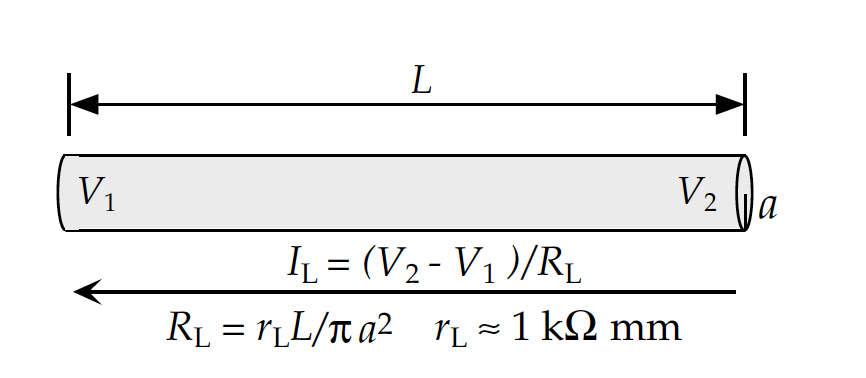
\includegraphics[width=0.5\textwidth]{./fig/Ra.png}
	\caption[Axiális ellenállás]{Az axiális ellenállás szemléltetése egy L hosszúságú kábelszakasz esetén. (Az ábrán $r_L = R_a$ jelölést használunk.) \textit{Forrás:}\cite{dayan2001theoretical} }
	\label{fig:Ra}
\end{figure}


\FloatBarrier
\paragraph{membrán kapacitás}
Fentebb szó volt arról, hogy a membrán úgy viselkedik mint egy kondenzátor. Ebben az esetben az azon felhalmozódó töltést $(Q)$ a következőképp számolhatjuk ki:

\begin{equation}\label{eq:Q}
	Q = C_m V 
\end{equation}
A kapacitás $(C_m)$ azt mondja meg, hogy adott feszültség mellett mennyi töltés halmozódik fel a kondenzátor fegyverzetein, azaz jelen esetben a sejtmembránon. A kapacitás arányos a felülettel, ezért érdemes a membrán tulajdonságait jobban jellemző, felületfüggetlen mennyiséget bevezetni, a specifikus membrán kapacitás:

\begin{equation}\label{eq:cm}
	c_m = \frac{C_m}{A_m}
\end{equation}
ahol $A_m$ a membrán felülete. Ez az érték tipikusan $1 \left[ \dfrac{\mu F}{cm^2}\right]$ nagyságrendbe esik.
Ha idő szerint lederiváljuk a~\ref{eq:Q} egyenlet mindkét oldalát, akkor megkapjuk a membránpotenciál megváltozását adott árambemenetre:

\begin{gather}\label{eq:dV}
	C_m \dfrac{dV}{dt} = \dfrac{dQ}{dt} \\
	\dfrac{dQ}{dt} = I
\end{gather}

\paragraph{membrán ellenállás}
Ahhoz is áram szükséges, hogy a membránpotenciált egy nem egyensúlyi szinten tartsuk. De ezt az áramot már a membrán ellenállás $(R_m)$ határozza meg a kapacitás helyett. Ugyanis Ohm-törvénye értelmében az $I_e$ befecskendezett áram eltolja a membrán potenciált egy $\Delta V$ értékkel:

\begin{equation}\label{eq:Rm}
	\Delta V = R_m I_e
\end{equation}
Ez a képlet csak kis $I_e$ áramok és $\Delta V$ feszültségek esetén érvényes, ha aktív idegsejtről beszélünk, mivel a membrán ellenállás ekkor a feszültség függvénye. Passzív esetben, amikor a membrán ellenállás nem feszültségfüggő, a fenti összefüggés általánosan igaz.
A membrán ellenállás nem más, mint a membrán konduktancia (áteresztőképesség) reciproka, ez pedig hasonlóan a membrán kapacitáshoz arányos a membrán felületével. A passzív membrán konduktancia tehát így írható fel:
\begin{equation}\label{eq:gpas}
	g_{pas} = \dfrac{1}{R_m A} = \dfrac{1}{r_m}
\end{equation}
amelynek tipikus értéke $g_{pas} = 0.0001 \left[\dfrac{\mu S}{cm^2}\right]$ körül mozog.

\paragraph{membrán időállandó}\label{par:tau}
Ha a membránkapacitást és membránellenállást összeszorozzuk akkor egy idő dimenziójú értéket kapunk. Ezt nevezzük a membrán idő állandónak, ami megadja a neurális folyamatok tipikus időskáláját:

\begin{equation}
	\tau_m = C_m R_m \approx \left(10-100\right) \left[ ms \right]
\end{equation}

\paragraph{membránáram}
Ha a membrán összes csatornáján átáramló áramot leosztjuk a membrán felületével, akkor megkapjuk az egységnyi felületre eső membrán áramot $(i_m)$. Passzív idegsejt esetében ez a nem feszültségfüggő (passzív) ion-csatornákból származik. Ezt a jelenséget a membrán passzív konduktanciájával jellemezzük és az ebből fakadó egységnyi felületre eső membránáramot a következőképpen írhatjuk le:

\begin{equation}\label{eq:im}
	i_m = g_{pas}\left( V-E_{pas}\right)
\end{equation}
ahol $g_{pas}$ a membrán passzív áteresztőképessége (konduktanciája) és $E_{pas}$ pedig a megfordítási potenciálja, ami passzív esetben épp az idegsejt nyugalmi potenciálja: $(E_{pas} = V_{m})$. Ezt az értéket meghaladva az ionok ellenkező irányba kezdenek folyni.











\subsection{Egykompartmentumos modell}\label{sec:single-comp}
Egyetlen paraméterrel írjuk le a membránpotenciált, azaz azt tételezzük fel hogy a membrán mentén állandó a potenciálkülönbség. Ez a közelítés egy szómára (egykompartentumos modell) teljesen helytálló, mert könnyen szétterjed benne az áramimpulzus. Tulajdonképpen arról van szó, hogy pontszerűnek tételezzük fel a szómát.
A passzív egykompartmentumos modell leírásához a~\ref{eq:dV} és a \ref{eq:im} egyenleteket kell összerakni:

\begin{equation}\label{eq:one_comp}
	c_m \dfrac{dV}{dt} = -g_{pas} \left( V-E_{pas} \right) + \dfrac{I_e}{A}
\end{equation}
ahol $I_e$ a kísérleti úton sejtbe juttatott áram (stimulus). A \ref{fig:single_comp} ábrán az egykompartmentumos modellek egy általános kapcsolási rajza látható. Vizsgálataink során ennek a modellnek mind a $c_m$ és a $g_{pas}$ (gyakran $g_L$-lel jelölik, mint például az itt fellelhető ábrákon is) paramétereinek az inferenciájával foglalkoztunk.

\begin{figure}[h!]
	\centering
	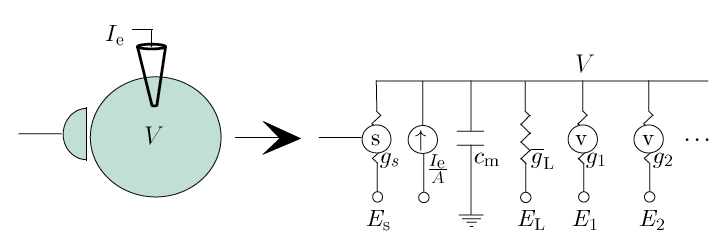
\includegraphics[width=0.7\textwidth]{./fig/single-compartment.png}
	\caption[Egykompartmentumos modell]{Egy általános egykompartmentumos modell, melyen a ion-csatornákból származó és az elektróda áram mellett még egy szinaptikus kapcsolat is van. \textit{Forrás:}\cite{dayan2001theoretical} }
	\label{fig:single_comp}
\end{figure}













\subsection{Térbelileg kiterjedt modellek}\label{sec:multi-comp}
A térbelileg kiterjedt modelleknél már nem tehetjük fel, hogy a membrán mentén a potenciál konstans, térbeli függést is feltételeznünk kell, melyet a kábelegyenlet ír le. Több elemből építjük fel az idegsejtet, melynek az egyes kompartmentumjaiban homogén a potenciál. Minél több részre osztjuk a sejtet, annál részletesebben tudjuk leírni a valós viselkedését. Ezt a folyamatot, vagyis a modellezés különböző szintjeit mutatja be szemléletesen a \ref{fig:multi_comp} ábra. Ez matematikailag összekapcsolt egykompartmentumos modellekkel írható le a következő módon (passzív idegsejt esetén):

\begin{equation}\label{eq:multi_comp}
\begin{split}
		c_m\dfrac{dV_\mu}{dt} = -g_{pas}\left(V_\mu - E_{pas}\right) + \dfrac{I_e^\mu}{A_\mu} + g_{\mu,\mu+1}\left(V_{\mu+1}-V_\mu \right) + g_{\mu,\mu-1}\left(V_{\mu-1}-V_\mu \right)
\end{split}
\end{equation}
ahol $I_e^\mu$ az adott $\mu$-edik kompartmentumba befecskendezett áram, $V_\mu$ a $\mu$-edik kompartmentum membránpotenciálja, $A_\mu$ a $\mu$-edik kompartmentum felülete. Ennek megfelelően $V_{\mu+1}$ és $V_{\mu-1}$ a jelenlegi komparmentumhoz csatlakozó másik kompartmentumok feszültségei. $g_{\mu,\mu+1}$ és $g_{\mu,\mu-1}$ a csatolási tényező, áteresztőképesség a kompartmentumok között, amelyre felírható a következő összefüggés:

\begin{equation}\label{eq:Ra}
	g_{\mu,\mu+1} = \dfrac{a}{2 R_a^{\mu,\mu+1} L^2}
\end{equation}
ahol $R_a$ a \ref{par:Ra}-paragrafusban említett axiális ellenállás, $a$ a kábel keresztmetszetének sugara és $L$ a kábel középpontjait összekötő szakasz hossza, ami ugyanakkora kábeldarabok esetén maga a kábelszakaszok hossza (a képlet erre az esetre érvényes). Inferencia során ezt a paramétert is becsültük, a kompartmentumok között állandónak tekintve ezt az értéket: 
\[ R_a^{\mu,\mu-1} = R_a^{\mu,\mu+1} = ... = R_a \]
Egy ilyen modellnek az általános kapcsolási rajza a \ref{fig:multi_comp_model} ábrán látható. 

Mi egy úgynevezett \textit{Ball and Stick} modellt építettünk vizsgálataink során, ami egy szómához kapcsolódó dendrit esetét reprezentálja. Ezen kívül használtunk egy kísérletből származó, bonyolult térbelileg kiterjedt morfológiát is. 

\begin{figure}[h!]
	\centering
	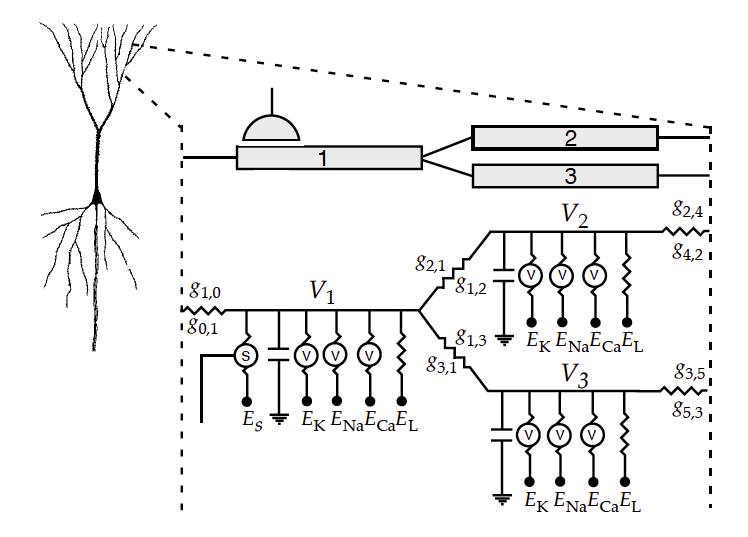
\includegraphics[width=0.7\textwidth]{./fig/multi-comp-model.png}
	\caption[Többkompartmentumos modell]{Egy kiterjedt idegsejt kompartmentumos modelljének kapcsolási rajza. Három kompartmentum látható, az elsőhöz szinaptikus bemenet kapcsolódik. Egy kompartmentumon háromféle ion által keltett áram van jelölve a megfelelő megfordulási potenciálok révén -- melyek feszültségfüggő ellenálláson keresztül kapcsolódnak --, illetve a \textit{"leak"} áram. A membránt pedig a kondenzátor helyettesíti. \textit{Forrás:}\cite{dayan2001theoretical}}
	\label{fig:multi_comp_model}
\end{figure}





\subsection{\textit{NEURON} idegsejt szimulációs program}
A munkánk során a \textit{Python} programozási nyelvet és környezetet használtunk. Az idegsejtek modellezésére, valamint a fentebb tárgyalt egyenletek numerikus megoldására pedig a \textit{NEURON} programot alkalmaztuk. Szerencsére ez betölthető a \textit{Python} környezetébe és így kommunikálni képes vele. Sok különböző paraméterkombinációval végzett szimuláció elvégzésénél ez nagy hasznunkra vált.

A \textit{NEURON} egy szimulációs környezet idegsejtek és komplex hálózatok modellezésére. Kényelmes eszközt szolgáltat modellek építéséhez, kezeléséhez és használatához. Kifejezetten jól alkalmazható esetekhez, melyek szorosan kapcsolódnak kísérleti adatokhoz. A \textit{NEURON "motorja"} különleges algoritmusokat használ annak érdekében, hogy az imént tárgyalt neurális tulajdonságokat leíró egyenleteket, minél hatékonyabban oldja meg. 

Munkánk során mi két modellt építettünk, egy egykompartmentumos -- ami egy neuronból áll -- és egy térbelileg kiterjedt úgynevezett \textit{Ball and Stick} modellt -- ami egy neuronból és egy hozzá csatlakozó dendritből áll. Ezen kívül egy valós kísérletből származó anatómiailag részletes modellre is alkalmaztuk megoldásainkat, melynek \textit{NEURON}-ba töltött rekonstrukciója látható a \ref{fig:morph}-ábrán.

\begin{figure}[h!]
	\centering
	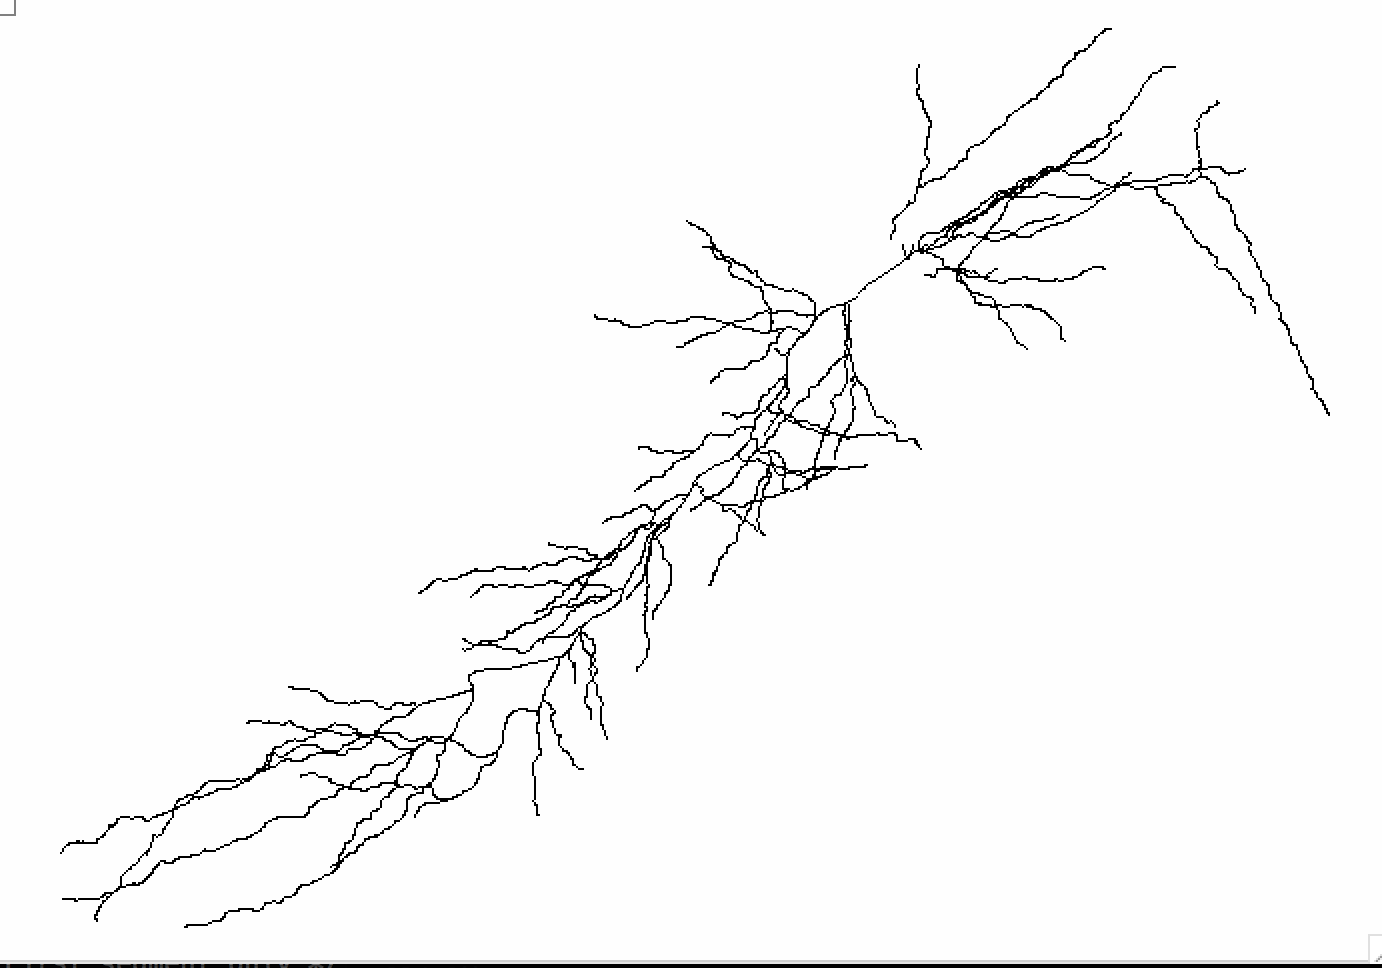
\includegraphics[width=0.5\textwidth]{./fig/morph.png}
	\caption[Kísérletből származó morfológia]{Egy valós idegsejt \textit{NEURON} programba töltött modellje.}
	\label{fig:morph}
\end{figure}


Az összes általunk használt modellt passzív idegsejti mechanizmus mellett vizsgáltuk. Ez azt jelenti, hogy az áramimpulzus hatására nem \textit{"tüzel"} az idegsejt, csak passzívan folyik belsejében az áram. Kísérletileg ezt bonyolult módon csatorna blokkolókkal lehet elérni, \textit{NEURON}-ban csupán beállítás kérdése.

Korábban láttuk, hogy hogyan is modellezünk egy biológiailag nagyon komplex idegsejtet: egyszerű elektronikából ismert hálózati elemekből összerakott modell nagyon jól visszaadja az empirikus megfigyeléseket. Ezek a vezetőképességen alapuló modellek az idegsejteknek a lehetséges legegyszerűbb biofizikai reprezentációi, melyekben az ion csatornákat ellenállásokkal, illetve a kettős lipid membránt pedig egy kapacitással helyettesítik (egy ilyen látható a~\ref{fig:fig1}. ábrán). Illetve az idegsejtet részegységekre (kompartmentumokra) bontjuk, melyek egy csatolt differenciál-egyenletrendszert szolgáltat. Az idegsejt ilyen jellegű modellezése, azaz kompartmentumos leírása látható a \ref{fig:multi_comp} ábrán. Analitikusan az idegsejt felosztásával tarthatunk a nullába, viszont numerikusan ez nem megoldható, véges kompartmentumokkal közelítünk.

\begin{figure}[h!]
	\centering
	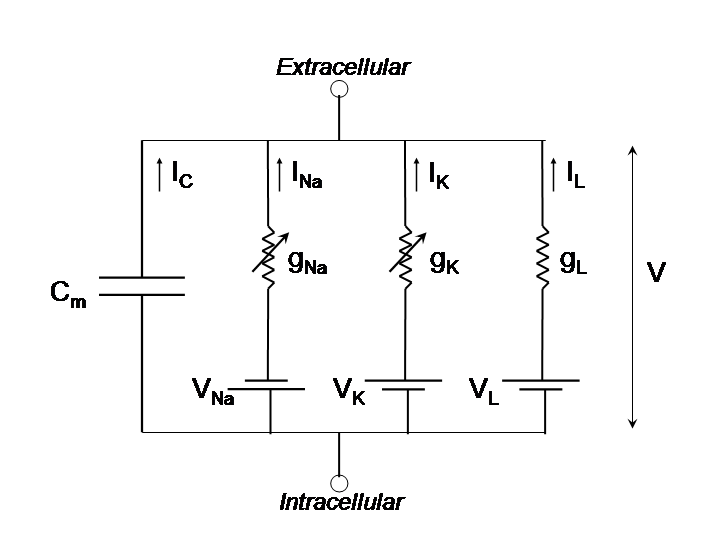
\includegraphics[width=0.6\textwidth]{./fig/Fig1.png}
	\caption[Idegsejt modell]{Példa az idegsejt konduktancián alapuló kapcsolási modelljéről. \\ \href{http://www.scholarpedia.org/w/images/e/eb/Fig1.png}{\textit{Forrás: http://www.scholarpedia.org/w/images/e/eb/Fig1.png}}}
	\label{fig:fig1}
\end{figure}

\begin{figure}[!h]
	\centering
	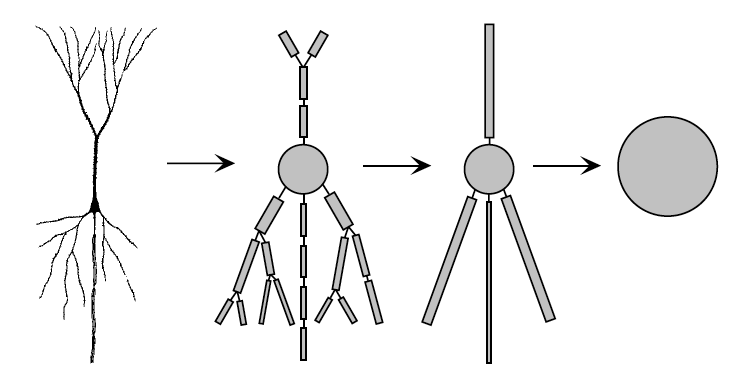
\includegraphics[width=0.6\textwidth]{./fig/multi-compartment.png}
	\caption[Többkompartmentumos modellezés]{\cite{dayan2001theoretical} Egy idegsejt különböző szintű kompartmentális modellezése. Jobbra haladva egyre inkább leegyszerűsítve írjuk le a sejtet.}
	\label{fig:multi_comp}
\end{figure}




\pagebreak
% Elmélet
\section{Megvalósítás}

%\pagebreak
% Eredmények
\section{Eredmények}
A vizsgálatok menete tipikusan úgy zajlik, hogy szintetikus \textit{"kvázi-kísérleti"} adatokat állítunk elő: Összeállítottunk két idegsejtmodellt -- egy egykompartmentumos, amely egyetlen szómából áll és egy \textit{"Ball and Stick"} modellt, amely pedig egy szómához csatlakozó dendritből áll -- és ennek az adott modellparaméterek melletti áramlépcső stimulusra adott válaszfüggvényére zajt  raktunk, így szimulálva a kísérleti adatokat. Majd ezekre az adatokra végeztük el a paraméterbecslést. Ezzel a módszerrel vizsgálni tudjuk az inferencia pontosságát, mert ismerjük a kiinduló, \textit{"igazi"} paramétereket. Minden esetben passzív idegsejtmodellekkel dolgoztunk.

Ugyanazokat a becsléseket -- új kezdeti paraméterek és zaj megvalósulásokra -- sokszor elvégeztük és a következő, inferencia minőségét jellemző statisztikákat állítottuk fel rájuk:
\begin{enumerate}
	\item \textbf{Eltérés \textit{(diff)}}: Az inferencia során becsült paraméter mennyire van távol az eredeti, kiindulási paramétertől.
	\item \textbf{Pontosság \textit{(acc)}}: A becsült paraméter poszterior eloszlásának maximuma (legvalószínűbbnek becsült paraméter valószínűsége, azaz maximális valószínűség) hányszorosa a kiindulási (eredeti) paraméterértékhez társított valószínűségnek: $p_{true}/p_{max}\cdot 100$.
	\item \textbf{Élesség \textit{(gain)}}: A poszterior eloszlás hányszor élesebb a priornál: $\Pi_{s}/P_s$. Ez természetesen akkor jellemzi a különböző eseteket, ha ugyanakkora prior eloszlással számolunk. Az eloszlás élességét úgy vizsgáljuk, hogy a görbe csúcsától a feléig veszünk egyenletesen $50$ magasságpontot -- illetve függvényértéket $y$ --, amikhez tartozó $x$-értékek -- ebből kettő van ideális esetben, mert a normál eloszlás szimmetrikus -- távolságát összegezzük, majd normáljuk $50$-el az eredményt.
	Ez az egyik legfontosabb jellemző, mert arra nyújt betekintést, hogy a mérés mennyi új információt hordozott.
%	\item \textbf{Laposság \textit{(broadness)}}: $P_{s}/\Pi_s\cdot 100$. Ezt az mennyiséget azért érdemes bevezetni, mert nagyon kis $P_s$ értékeknél az élességhez tartozó érték \textit{"elszáll"}, így nagy lesz a szórása. Szemléletesen azt jelenti, hogy ha ez az érték $100\%$ akkor a poszteriorom épp olyan mint a priorom, tehát nem nyertem ki új információt a kísérletből.
\end{enumerate}

Ezeket a statisztikákat elvégeztük különböző modellekre -- különböző zajmodellek mellett -- és kísérleti protokollokra, melynek eredményeit a következő pontokban részletezzük. Végezetül valódi kísérleti adatokra is alkalmaztuk a paraméterbecslési eljárásunkat, valamint vizsgáltuk a kísérleti zaj tulajdonságait.



\subsection{Egykompartmentumos modell}
Először a \ref{sec:single-comp}-fejezetben tárgyalt passzív egykompartmentumos modellre alkalmazzuk a megoldásainkat. Egy pontszerű szómát ingerlünk áramimpulzus bemenettel, valamint mérjük a feszültségválaszát. Ennek szemléltetése látható a \ref{fig:point}-ábrán.

\begin{figure}[h!]
	\centering
	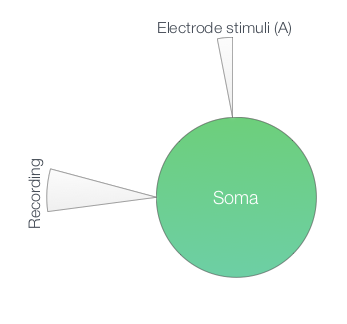
\includegraphics[width=0.4\linewidth]{fig/models/point}
	\caption[Egykompartmentumos modell szemléltetése]{Egykompartmentumos modell szemléltető ábrája. Egyetlen pontszerű -- nincs térbeli kiterjedés -- szómát stimulálunk az elektróda árammal és mérjük a feszültségválaszát.}
	\label{fig:point}
\end{figure}

Egy $175 \left[ms\right]$-on keresztül injektált $0.1 \left[mA\right]$ áramerősség stimulusú -- és passzív biofizikai beállítású -- protokollt alkalmaztunk az alábbiakban. Továbbá a fehér zaj szórásának mindenhol $\sigma_w = 7\left[mV\right]$-ot választottunk. Hasonló beállításokkal előállított adatsor tekinthető meg a korábbi \ref{fig:white}-ábrán. Színes zaj szórásának pedig $\sigma_\epsilon = \sqrt{3} \left[mV\right]$-ot és az időbeli korreláció lecsengési idejét jellemző karakterisztikus idejének pedig $\tau=10 \left[ms\right]$-ot. Ezt szemlélteti a korábbi \ref{fig:colored}-ábra.

\subsubsection{Fehér zaj}
\paragraph{egy paraméter}
Az a kérdés, hogy passzív egykompartmentumos modell áramlépcső stimulusra adott feszültségválasza segítségével, milyen pontosan tudunk egy paramétert -- jelen esetben a $cm$ membránkapacitás paraméterét -- becsülni.

Az eredmények a \ref{fig:wn1}-ábrán láthatóak. A legfontosabb jellemző mennyiség az élesség, amely jelen esetben $2.75$-nek adódott. Ez azt jelenti, hogy szimulációk során a poszterior eloszlás átlagosan $2.75$-ször élesebb (hegyesebb) volt a prior eloszlásnál. A mérés után ennyi új információra tehetünk szert az adott paraméterre nézve.


\paragraph{két paraméter}
Itt azt vizsgáljuk, hogy együtt inferálva $cm$ paramétert egy másik ($g_{pas}$) paraméterrel, az mennyire befolyásolja a $cm$ becslését.

A \ref{fig:wn2_joint}-ábrán látható egy futtatás tipikus eredménye a két paraméter együttes poszterior eloszlására. Ebből látszódik, hogy $g_{pas}$ paraméter nagyon pontosan becsülhető, ennek következtében nem rontja le a másik ($cm$) paraméter becslését. Másképp fogalmazva az együttes eloszlás, szinte épp maga a $cm$ paraméter marginális eloszlása. 


A \ref{fig:wn2}-ábrán látható a sok futtatás eredményéből származó marginális eloszlások és statisztikák mindkét paraméterre. Ezeken látszódik, hogy $g_{pas}$ paraméter eloszlása tényleg nagyon éles, a priorjánál $15.87$-szer élesebb a poszteriorja. Tehát ezt a paramétert pontosan tudjuk becsülni. Továbbá az is látható, hogy a $cm$ paraméter marginális poszterior eloszlásának alakja valóban lényegesen nem változott, nem romlott a becslés pontossága -- a fentebbi meggondolásokkal egybevágóan.

\subsubsection{Színes zaj}
A kétparaméteres becslést exponenciálisan lecsengő autokorrelációval rendelkező színes zaj esetére is elvégeztük. Azt várjuk, hogy a becslés pontossága csökkenni fog, mivel az adatpontok nem függetlenek, így kevesebb effektív mintavételi pontunk van -- még akkor is, ha növeljük az időbeli felbontását.

A paraméterek együttes eloszlása a \ref{fig:cn1_joint}-ábrán láthatóak. Összehasonlítva a fehér zajos esettel ez tényleg kevésbé éles. A \ref{fig:cn1}-ábrán pedig a sok szimuláció átlagos, egyes paraméterekre marginalizált eredménye látható.

Az eredmények azt mondják, hogy valóban pontatlanabb a becslés színes zaj esetén, hiszen mindkét paraméter \textit{élessége} csökkent: $cm$-nek $1.92$ és $g_{pas}$-nak pedig $7.66$. És mindezt úgy, hogy ráadásul kisebb ($\sigma_\epsilon = \sqrt{3} \left[mV\right]$) szórást alkalmaztunk mint fehér zajnál ($\sigma_w = 7\left[mV\right]$)!

\begin{figure}[h!]
	\centering
	\subfloat[Illusztráció]{{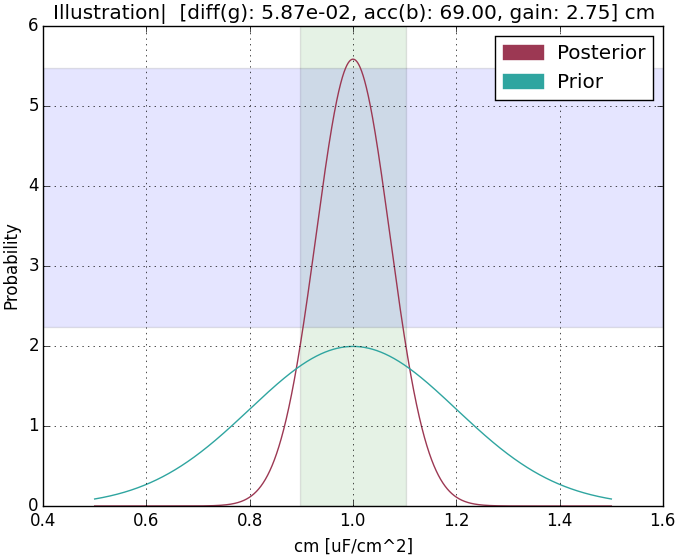
\includegraphics[width=0.5\textwidth]{./fig/wn1/illustration_cm.png} }}
	\subfloat[Élesség]{{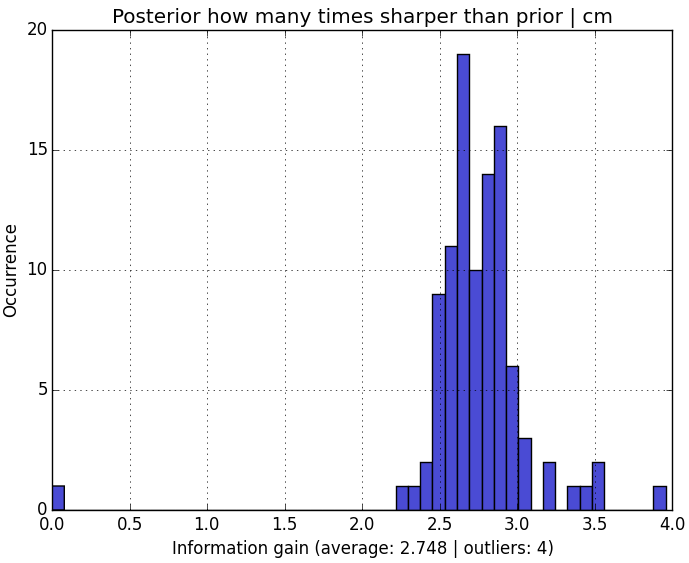
\includegraphics[width=0.5\textwidth]{./fig/wn1/igain_cm.png} }}
	\\	
	\subfloat[Eltérés]{{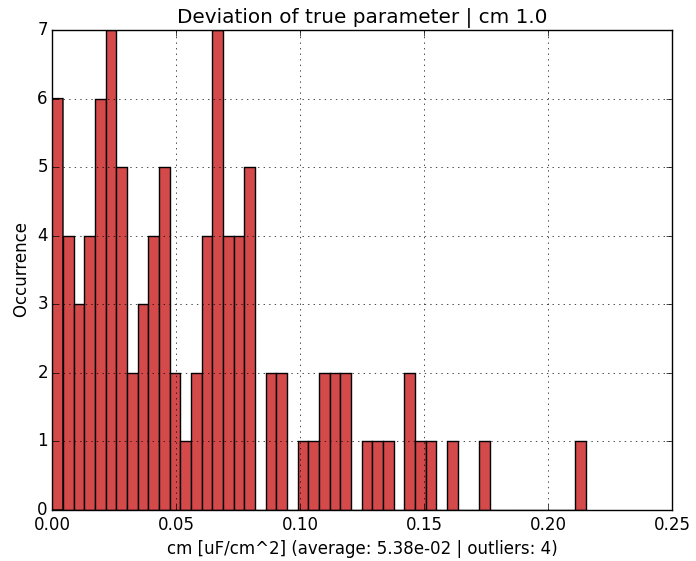
\includegraphics[width=0.5\textwidth]{./fig/wn1/deviation_cm.png} }}
	\subfloat[Pontosság $(p_{max}/p_{true}\cdot 100)$]{{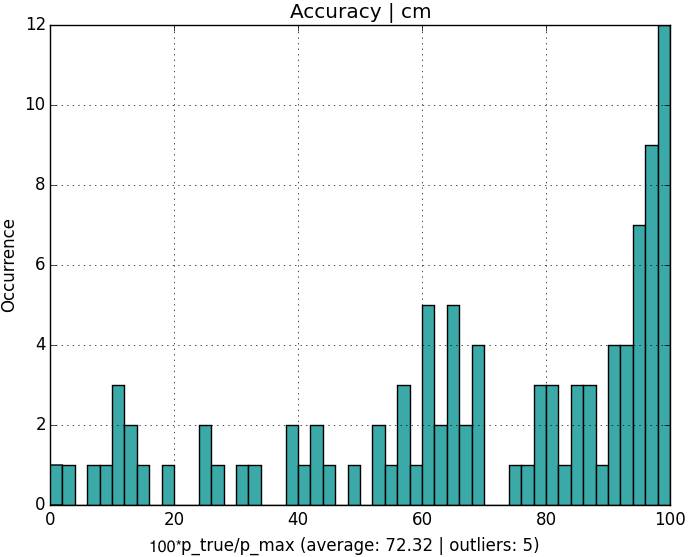
\includegraphics[width=0.5\textwidth]{./fig/wn1/accuracy_cm.png} }}
	\caption[Egy kompartmentum, egy paraméter, fehér zaj eredmény és ábratípus magyarázat]{$100$ db szimuláció összefoglaló ábrái az egyparaméteres, fehér zajos becsléshez. Az \textbf{(a)} rész illusztrálja a szimulációk során előforduló átlagos poszterior alakot, valamint egyéb statisztikákat is feltüntet: A fejlécen láthatóak (sorban) az \textbf{eltérés}(diff), \textbf{pontosság}(acc) és \textbf{élesség}(gain) átlagos értékei. Továbbá a függőleges zöld sáv azt jelzi, hogy a valódi érték milyen tartományban mozgott, ha ezt a poszteriort kaptuk. Vagy épp ellenkezőleg úgy is felfoghatjuk, hogy ha a prior csúcsánál van a valódi érték, akkor a becsült poszterior maximuma a zöld sávban mozgott szimulációk során. Végül a vízszintes kék sáv azt mutatja, hogy a valódi értékekhez milyen valószínűségeket rendelt a poszterior általában -- ez konzisztens az előzővel. Az előbbiek szépen szemléltetik a valószínűségi felfogást: a poszterior alatti tartományomban lesz valahol az igazi érték, de nem biztos, hogy a maximális valószínűségnél. \textbf{(b)}, \textbf{(c)} és \textbf{(d)} ábrarészleteken pedig az előbbi értékek hisztogramos ábrázolása látható.}
	\label{fig:wn1}
\end{figure}

%\begin{figure}[h!]
%	\centering
%	\subfloat[Fehér zajos együttes eloszlás]{{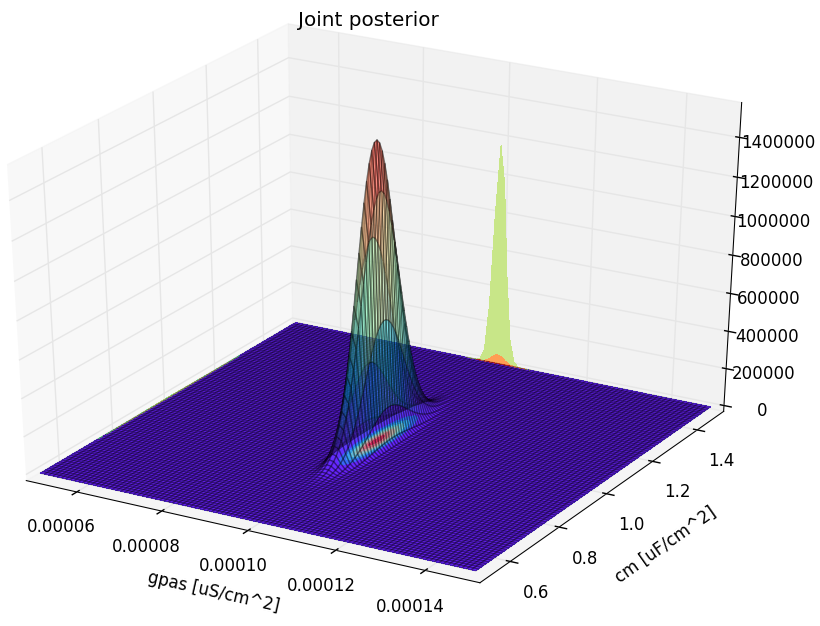
\includegraphics[width=0.5\textwidth]{./fig/wn2/JointP_cm_gpas(1).png} }}
%	\subfloat[Színes zajos együttes eloszlás]{{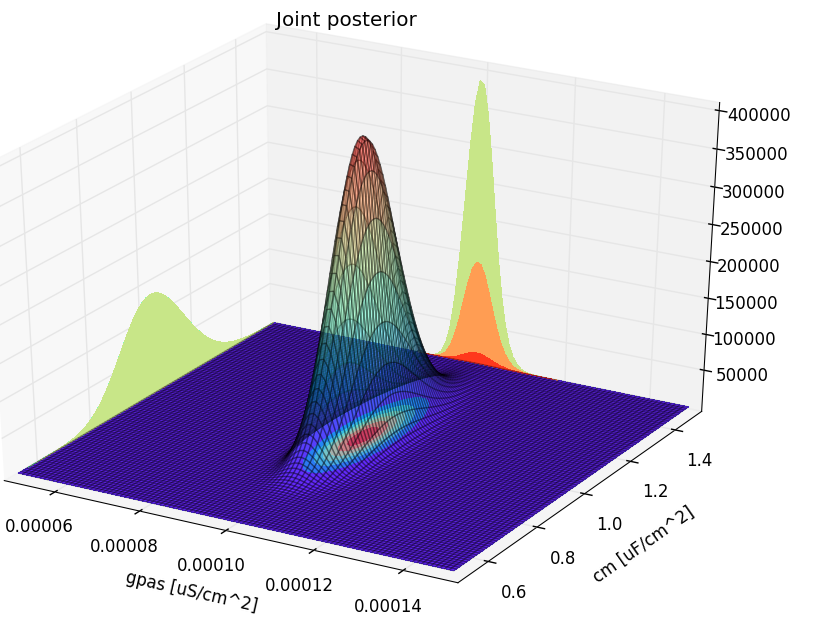
\includegraphics[width=0.5\textwidth]{./fig/cn1/JointP_cm_gpas(1).png} }}
%	\caption[(Egy kompartmentum két paraméter, fehér zaj eredmény]{\textbf{(a):} Egy futtatásból származó kétparaméteres, fehér zajos inferencia együttes eloszlása. Láthatóan $g_{pas}$ paramétert nagyon pontosan tudjuk becsülni, $cm$ paramétert pedig kevésbé. \textbf{(b): Előbbihez hasonló }}
%	\label{fig:joints}
%\end{figure}


\begin{figure}[h!]
	\centering
	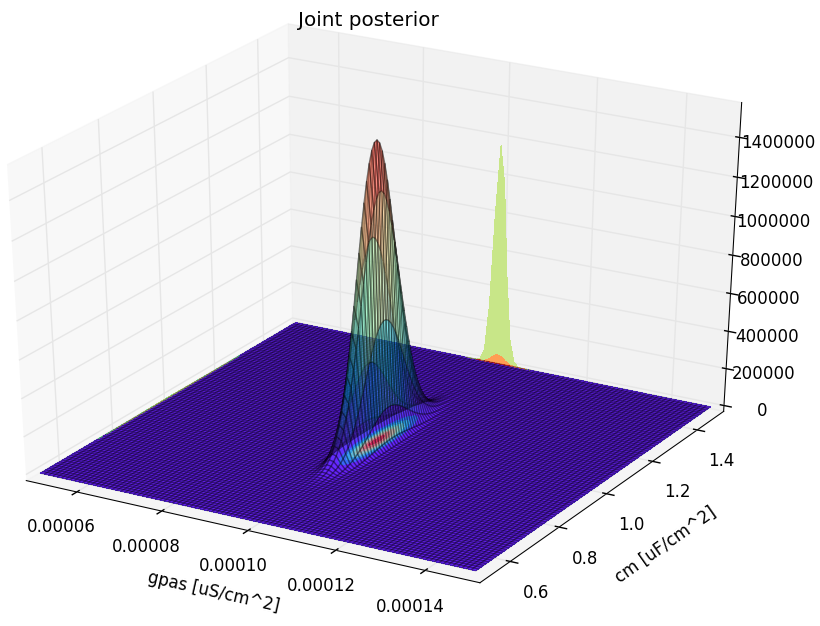
\includegraphics[width=0.8\linewidth]{fig/wn2/JointP_cm_gpas(1).png}
	\caption[Egykompartmentumos modell fehér zaj együttes poszterior eloszlása]{Egy futtatásból származó kétparaméteres, fehér zajos becslés együttes eloszlása. Láthatóan $g_{pas}$ paramétert nagyon pontosan tudjuk becsülni, $cm$ paramétert pedig kevésbé.}
	\label{fig:wn2_joint}
\end{figure}


\begin{figure}[h!]
	\centering
	\subfloat[$cm$ paraméter]{{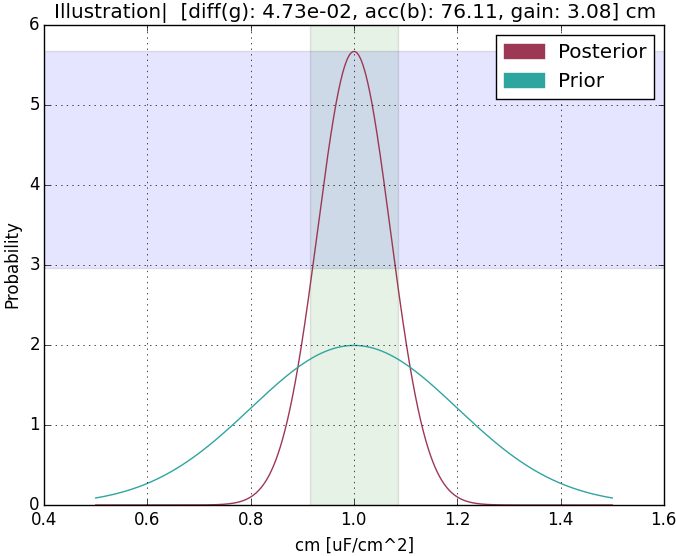
\includegraphics[width=0.5\textwidth]{./fig/wn2/illustration_cm.png} }}
	\subfloat[$g_{pas}$ paraméter]{{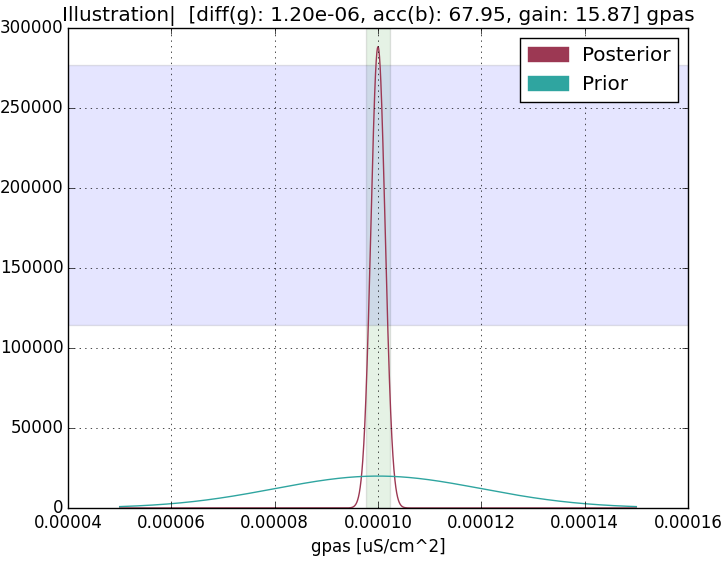
\includegraphics[width=0.5\textwidth]{./fig/wn2/illustration_gpas.png} }}
	\caption[Egy kompartmentum két paraméter, fehér zaj eredmény]{$100$ db szimuláció összefoglaló ábrái a kétparaméteres, fehér zajos becslésre, külön mind a két paraméterre. Ezek már a szimuláció során előforduló, átlagos marginális poszterior eloszlásalakok az egyes paraméterekre.}
	\label{fig:wn2}
\end{figure}


\begin{figure}[h!]
	\centering
	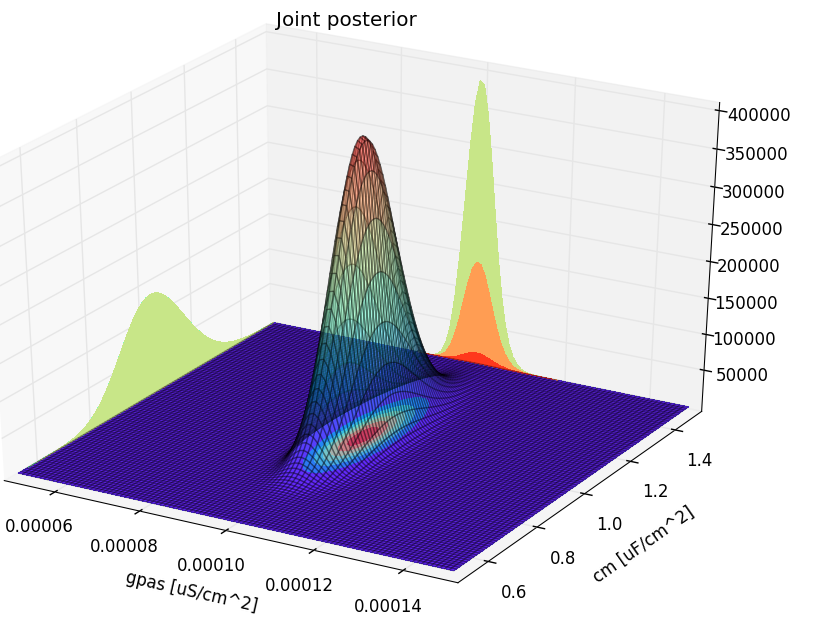
\includegraphics[width=0.8\linewidth]{fig/cn1/JointP_cm_gpas(1).png}
	\caption[Egykompartmentumos modell, színes zaj, együttes poszterior eloszlása]{Egy futtatásból származó kétparaméteres, színes zajos becslés együttes eloszlása. Látható, hogy a paramétereket kevésbé pontosan tudjuk becsülni, mint a fehér zajos esetben.}
	\label{fig:cn1_joint}
\end{figure}

\begin{figure}[h!]
	\centering
	\subfloat[$cm$ paraméter]{{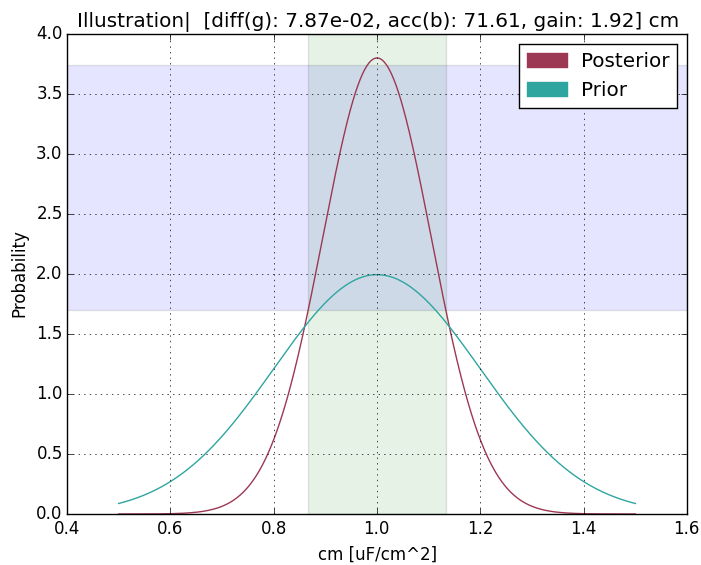
\includegraphics[width=0.5\textwidth]{./fig/cn1/illustration_cm.png} }}
	\subfloat[$g_{pas}$ paraméter]{{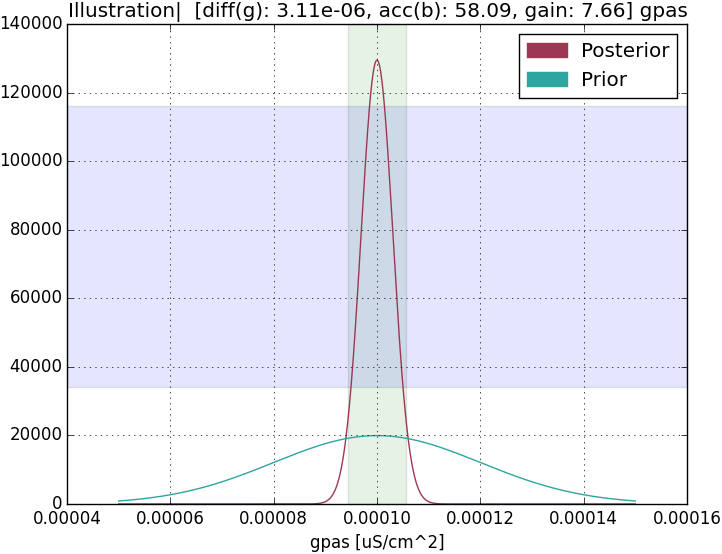
\includegraphics[width=0.5\textwidth]{./fig/cn1/illustration_gpas.png} }}
	\caption[Egy kompartmentum, két paraméter, színes zaj eredmények]{$100$ db szimuláció összefoglaló ábrái a kétparaméteres, színes zajos becslésre, külön mind a két paraméterre. Ezek már a szimuláció során előforduló, átlagos marginális poszterior eloszlásalakok, az egyes paraméterekre.}
	\label{fig:cn1}
\end{figure}




\clearpage
\subsection{Térbelileg kiterjedt modell: \textit{Stick and Ball}}
A \ref{sec:multi-comp}-fejezetben tárgyalt térbelileg kiterjedt, többbkompartmentumos passzív idegsejtmodellekre is alkalmaztuk a módszerünket. Pontosabban a \textit{Ball and Stick} modellre, amely egy szómához csatlakozó dendritből áll. A szómába injektáltuk az elektróda áramot és azon is mértünk. Ennek szemléltetése látható a \ref{fig:spatial}-ábrán.

\begin{figure}[h!]
	\centering
	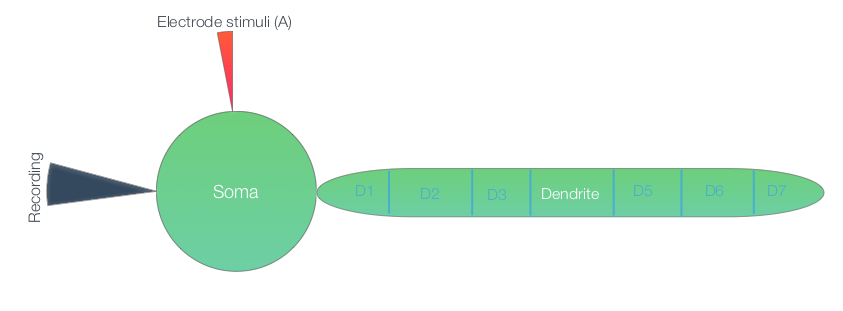
\includegraphics[width=0.9\linewidth]{fig/models/spatial}
	\caption[Többkompartmentumos modell szemléltetése]{Térbelileg kiterjedt, \textit{Stick and Ball} modell szemléltető ábrája. Egy szómához csatlakozik egy dendrit, melyet kisebb kompartmentumokra bontunk ($D1,D2,...$). A szómát ingereljük és azon is végzünk mérést.}
	\label{fig:spatial}
\end{figure}

Az $R_a$ és $g_{pas}$ paramétereket becsüljük együtt. Azt várjuk, hogy a dendritere jellemző passzív paraméter ($R_a$), azaz a fajlagos axiális ellenállás meghatározása kevésbé pontos lesz, tisztán a szómán végzett mérésekből, előzetes ismereteink alapján.

Itt is egy $175 \left[ms\right]$-on keresztül injektált $0.1 \left[mA\right]$ áramerősség stimulusú protokollt alkalmaztunk, ugyancsak passzív biofizikai és hasonló zaj beállításokkal.


\subsubsection{Fehér zaj}
Hasonlóan az előző pontokban látottakhoz, erre az összeállításra is lefuttattuk a szimulációkat. Az egy futtatásból származó tipikus együttes likelihood függvény és poszterior eloszlás látható a \ref{fig:wn3_joint}-ábrán, valamint a sok futtatás eredménye pedig a \ref{fig:wn3}-ábrán.

Az eredmények teljesen kielégítik az elvárásainkat: az $R_a$ paraméter tényleg rosszul becsülhető tisztán az idegsejten végzett mérésekből és ez egyben (valamennyivel) rontja $g_{pas}$ paraméter becslését is. Az együttes eloszlások ábrájáról látszódik jól, hogy ez miért történik: az $Ra-gpas$ paramétersíkra levetített ellipszisek kissé \textit{"ferdék"}, így $R_a$ tengelyre kiösszegezve az eloszlást, $g_{pas}$ marginális eloszlása kiszélesedik. Előfordulhat olyan eset, hogy az egyik paramétert rosszul tudjuk becsülni, viszont ez a másikat nem rontja el -- tehát a paraméterek nem \textit{"korrelálnak"} --, akkor ha a levetített ellipszisek nem ferdék.


\begin{figure}[h!]
	\centering
	\subfloat[együttes likelihood]{{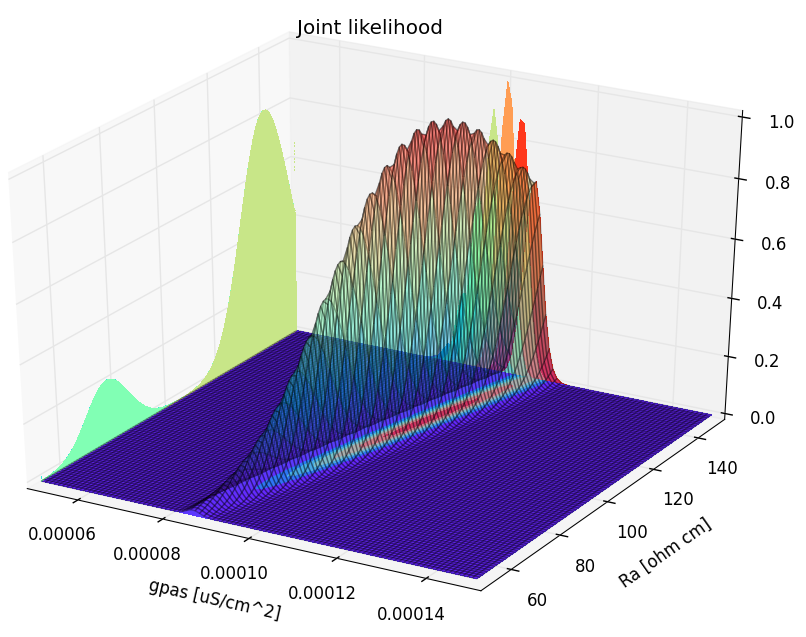
\includegraphics[width=0.5\textwidth]{./fig/wn3/JointL_Ra_gpas(0).png} }}
	\subfloat[együttes poszterior]{{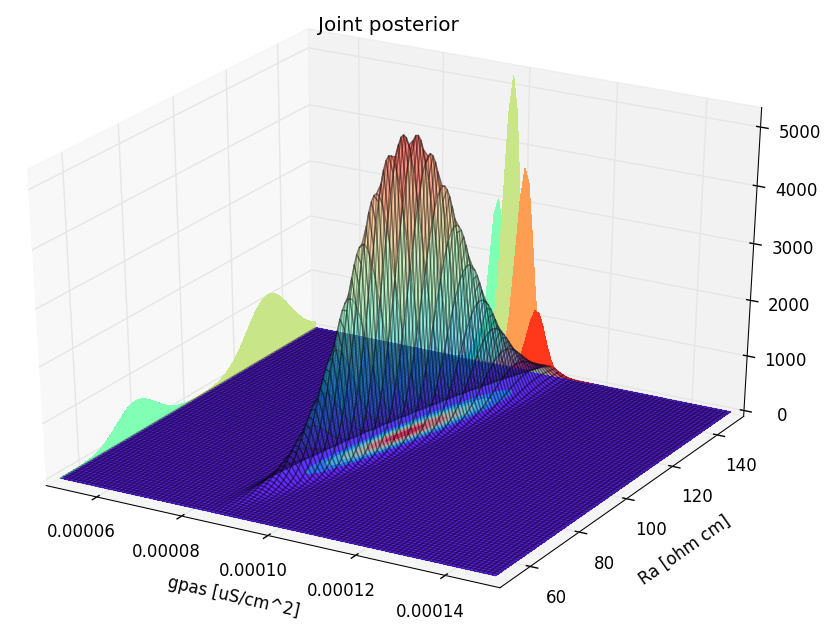
\includegraphics[width=0.5\textwidth]{./fig/wn3/JointP_Ra_gpas(0)} }}
	\caption[\textit{Stick and ball}, két paraméter, fehér zaj együttes eloszlásai]{Egy (fehér zajos) futtatásból származó likelihood(a) és poszterior(b). Szépen látszódik, hogy az $R_a$ paraméter becslése tényleg pontatlan, míg a $g_{pas}$ továbbra is viszonylag éles.}
	\label{fig:wn3_joint}
\end{figure}


\begin{figure}[h!]
	\centering
	\subfloat[$R_a$ paraméter]{{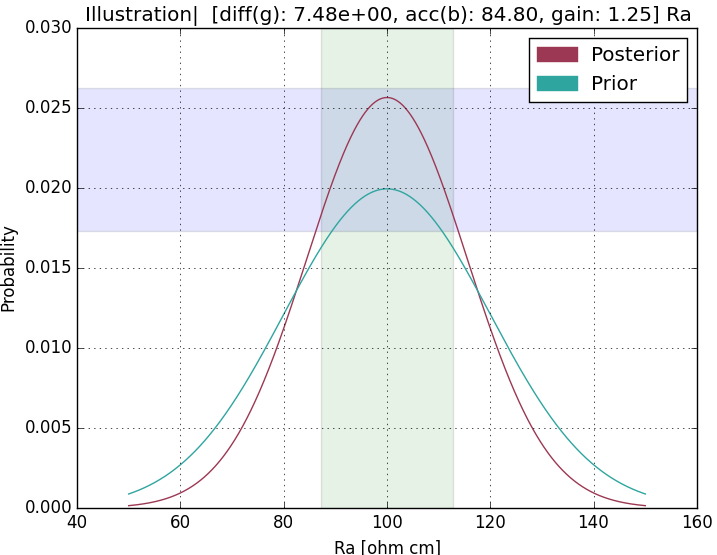
\includegraphics[width=0.5\textwidth]{./fig/wn3/illustration_Ra.png} }}
	\subfloat[$g_{pas}$ paraméter]{{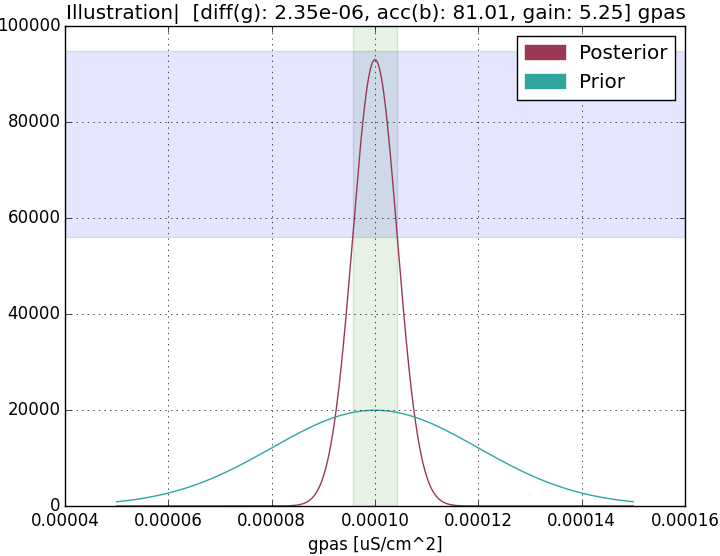
\includegraphics[width=0.5\textwidth]{./fig/wn3/illustration_gpas.png} }}
	\caption[\textit{Stick and ball}, két paraméter, fehér zaj eredmény]{$100$ db szimuláció összefoglaló ábrái, fehér zaj esetére. A szimuláció során előforduló, átlagos marginális poszterior eloszlásalakok az egyes paraméterekre.}
	\label{fig:wn3}
\end{figure}

\subsubsection{Színes zaj}
Színes zaj esetén is lefuttattuk a szimulációkat. Azt várjuk, hogy a becslés pontossága tovább csökken. A \ref{fig:cn2_joint}-ábrán láthatóak az egy futtatásból származó együttes likelihood és poszterior eredmények. A likelihood ábrájáról látható, hogy az $R_a$ paramétert becslése tulajdonképpen nem is működik, \textit{"elszáll" }. Eredetileg $R_a \approx 100 \left[\Omega cm\right]$ értékből indultunk ki (ezzel az értékkel generáltuk a szintetikus adatot), viszont az inferencia azt mondja, hogy $R_a$ paraméter tart a végtelenbe. Tehát a zaj bizonyos esetekben úgy torzítja az eredményt, hogy $R_a = \infty$ adódik, ami azt jelenti, hogy a dendrit lecsatolódik és a modell egykompartmentumúként funkcionál. Továbbá ismét látszódik, hogy a két paraméter együttese -- a két paraméter egymással kölcsönhatva -- határozza meg a modell jó illeszkedését.

A \ref{fig:cn2}-ábrán pedig a sok futtatás átlagos eredménye látható. Az ábráról az olvasható le, hogy $R_a$ élessége $1.05$, tehát lényegében nem nyertünk ki információt a mérésből erre a paraméterre vonatkozóan. Ez a marginális poszterior alakjából is látszódik, ami szinte rásimul a priorra. 

\begin{figure}[h!]
	\centering
	\subfloat[együttes likelihood]{{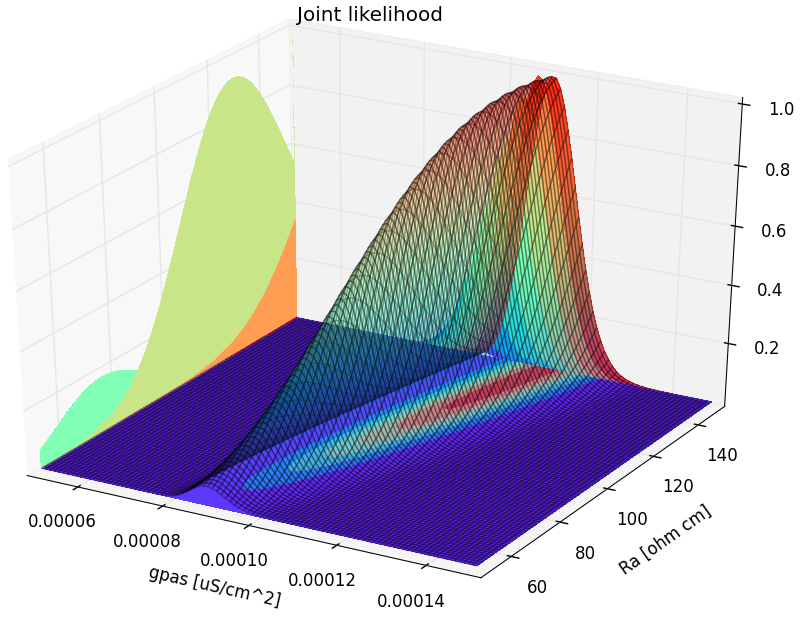
\includegraphics[width=0.5\textwidth]{./fig/cn2/JointL_Ra_gpas(1).png} }}
	\subfloat[együttes poszterior]{{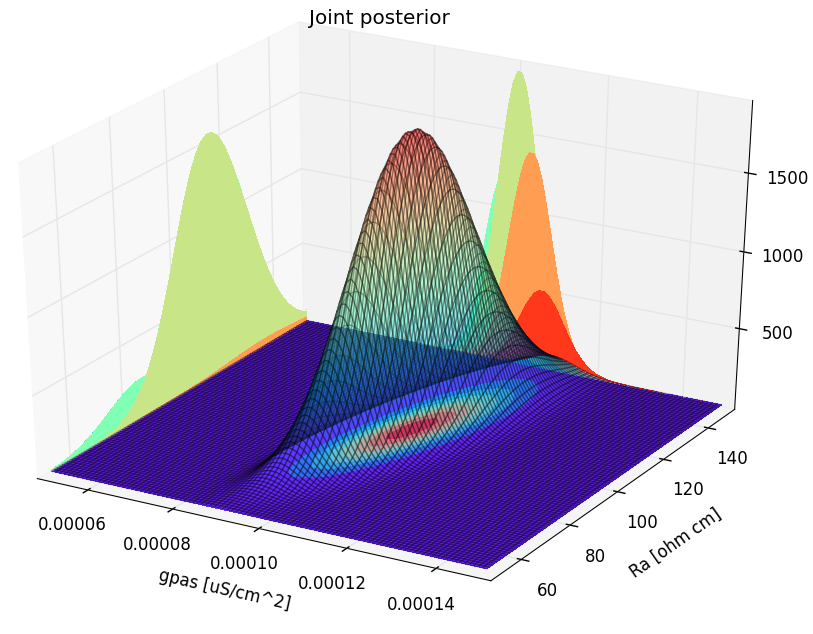
\includegraphics[width=0.5\textwidth]{./fig/cn2/JointP_Ra_gpas(1)} }}
	\caption[\textit{Stick and ball}, két paraméter, színes zaj együttes eloszlásai]{Egy (színes zajos) futtatásból származó likelihood(a) és poszterior(b). Látható, hogy tovább romlik a becslés pontossága, valamint hogy a paraméterek egymással kölcsönhatva határozzák meg a modell jó illeszkedését.}
	\label{fig:cn2_joint}
\end{figure}


\begin{figure}[h!]
	\centering
	\subfloat[$R_a$ paraméter]{{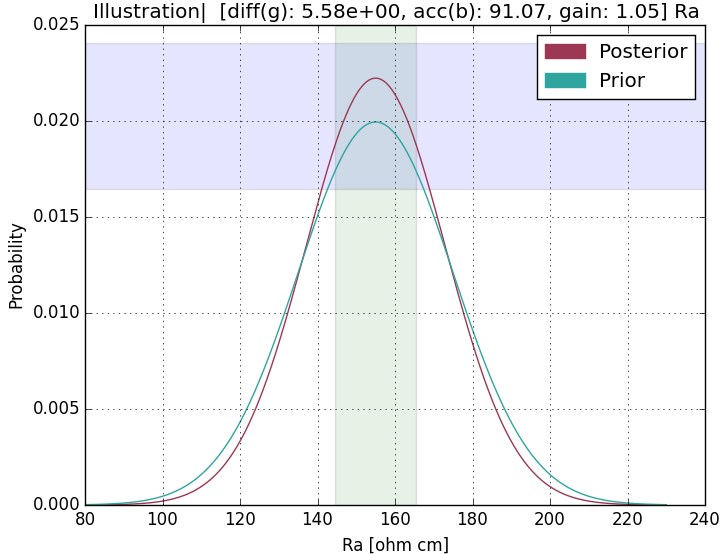
\includegraphics[width=0.5\textwidth]{./fig/cn2/illustration_Ra.png} }}
	\subfloat[$g_{pas}$ paraméter]{{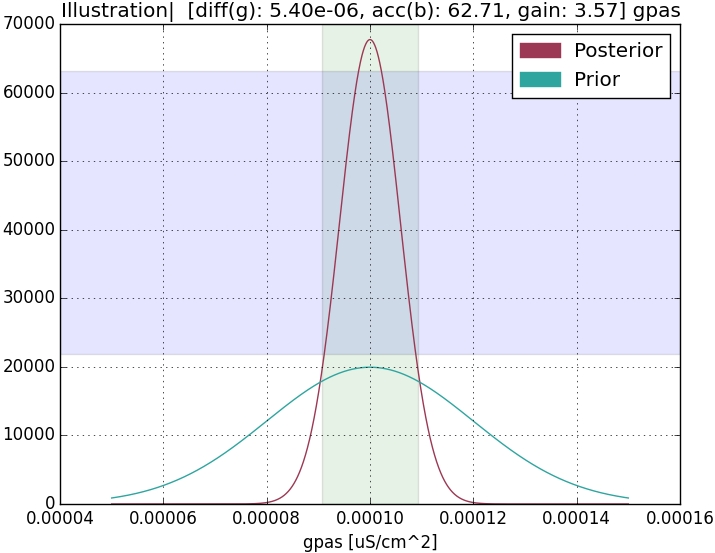
\includegraphics[width=0.5\textwidth]{./fig/cn2/illustration_gpas.png} }}
	\caption[\textit{Stick and ball}, két paraméter, színes zaj eredmény]{$100$ db szimuláció összefoglaló ábrái, színes zaj esetére. A szimuláció során előforduló, átlagos marginális poszterior eloszlásalakok az egyes paraméterekre.}
	\label{fig:cn2}
\end{figure}


\FloatBarrier
\clearpage
\subsection{Kísérleti protokollok információtartalma}
Ebben a részben azt vizsgáljuk, hogy különböző alakú áramimpulzusok, illetve azok kombinációi hogyan hatnak ki a paraméterbecslés pontosságára, tehát különböző kísérleti protokollokat hasonlítunk össze. Ezt elvégeztük ismét több esetben: a két zajtípusra és idegsejtmodellre. Az eredmények a két zajtípus esetén összhangban voltak. Most csak az egykompartmentumos modell, színes zaj melletti eredményeit közöljük, mert ezzel szemléltethető jól a módszerünk hatékonysága.

Három különböző idegsejt ingerlésű protokollt készítettünk és hasonlítottuk őket össze módszerünkkel. Név szerint (a) egy \textit{hosszú és kicsi} amplitúdójú -- épp amilyennel eddig dolgoztunk az előző pontokban --, (b) egy \textit{rövid és nagy} amplitúdójú, valamint ezek kombinációjából létrejövő (c) \textit{hosszú-rövid} áramimpulzus stimulusokat használtunk. A modell ezekre a stimulusokra adott determinisztikus feszültségválasza és az arra rakódott színes zaj látható a \ref{fig:protocol}-ábra első sorjában. Zaj szórásának a szokásos $\sigma_\epsilon = \sqrt{3} \left[mV\right]$-ot választottuk.

Az eredményeket a \ref{fig:protocol}-ábra illusztrálja. A jobb átláthatóság kedvéért, a poszterior élességének jellemző mennyiségét, az élességet összeszedtük a \ref{tab:res}-táblázatba. 

\begin{table}[h!]
	\centering
	\begin{tabular}{@{}|l|c|c|c|@{}}
		\toprule
		& \textit{hosszú} stimulus & \textit{rövid} stimulus & \textit{hosszú-rövid} stimulus \\ \midrule
		$cm$ \textit{gain}   & 1.75   & 5.1   & 5.01         \\
		$g_{pas}$ \textit{gain} & 7.02   & 2.62  & 7.21         \\ \bottomrule
	\end{tabular}
	\caption{Az eredmények táblázatba foglalva. Az egyes stimulusok esetén, a paraméterek becslésének pontosságát jellemző élesség (gain) értékeket láthatjuk.}
\label{tab:res}
\end{table}

Az eredmények alapján $cm$ paraméterre nézve a (b) típusú protokoll hordozta a több információt, az (a)-hoz képest. Ez abból következik, hogy ez a paraméter a tranziens ágakért felelős, így a gyorsan változó, nagy emelkedésű szakaszokkal lehet jól beállítani. 

A $g_{pas}$ paraméternél pedig épp ellenkezőleg, a különböző áraminjekcióhoz tartozó konstans szakaszok számítanak. Ezzel összhangban a módszerünk az (a) típusú protokollt találta jobbnak $g_{pas}$ paraméter becsléséhez.

Előbbieket, vagyis az (a) és (b) típusú stimulusokat kombinálva egy olyan protokoll hozható létre (c), amely egyszerre mindkét paramétert jól meg tudja határozni.

Megjegyzendő, hogy valószínűleg hasonló eredményt értünk volna el a (c) típusú protokolléhoz, ha a (b) típusú áramimpulzus amplitúdójának nagyságát használjuk az (a) típusú áramimpulzus időhosszával, hiszen ekkor ugyan azok a tranziens ágak jelentek volna meg és hasonlóan hosszú konstans szakasz. Viszont a sejtet tönkretehetjük, ha nagy áramerősséget injektálunk bele huzamosabb ideig, ezért célszerű szétbontani nagy amplitúdós rövid szakaszra és kis amplitúdós hosszú szakaszra, hogy mindkét paramétert pontosan tudjuk becsülni.
%
%\begin{figure}[h!]
%	\centering
%	\subfloat[hosszú áramimpulzusre adott válasz]{{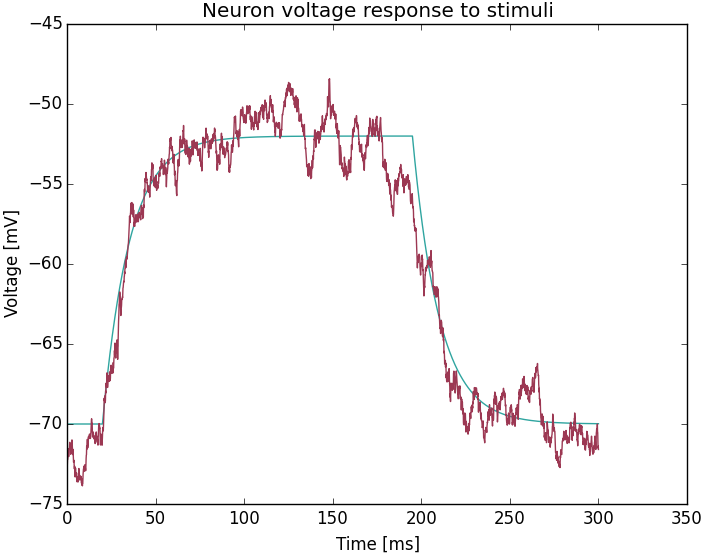
\includegraphics[width=0.37\textwidth]{./fig/Protocol/stims/broad_noised} }}
%	\subfloat[rövid áramimpulzus adott válasz]{{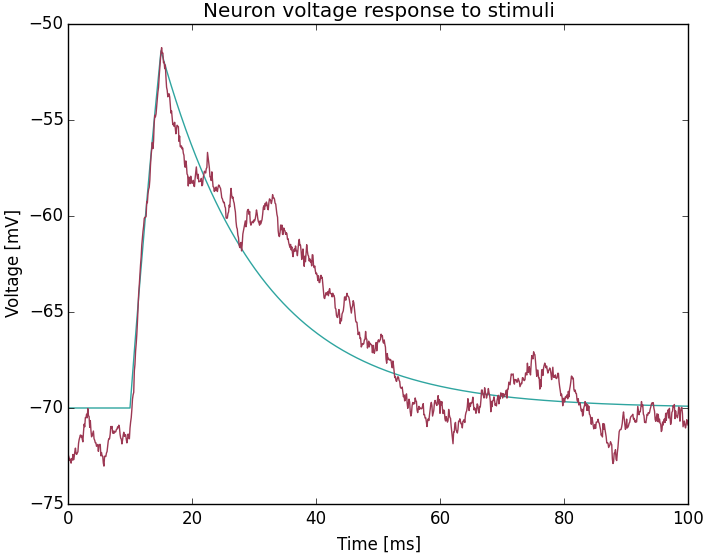
\includegraphics[width=0.37\textwidth]{./fig/Protocol/stims/narrow_noised} }}
%	\subfloat[hosszú-rövid áramimpulzusra adott válasz]{{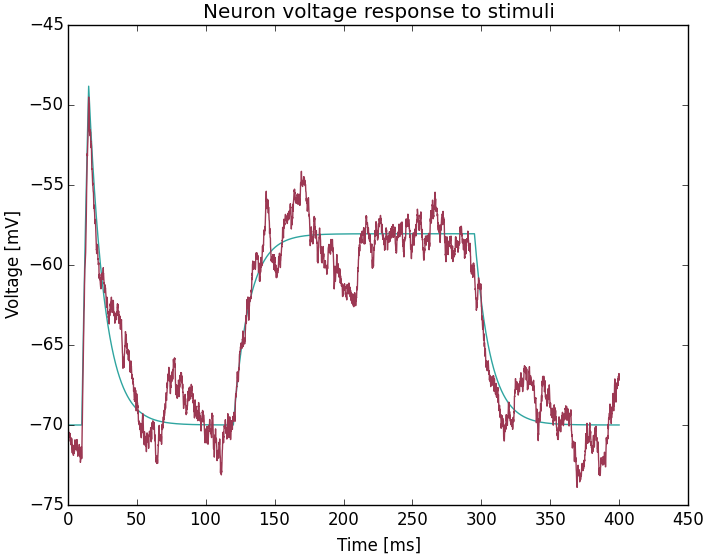
\includegraphics[width=0.37\textwidth]{./fig/Protocol/stims/both_noised} }}
%	\caption[Különböző stimulusra adott sejtválaszok]{Egykompartmentumos modell különböző áramimpulzusra adott feszültségválaszai láthatóak kékkel, valamint az erre rakott színes zajból előálló szintetikus adatok pirossal. }
%	\label{fig:stims}
%\end{figure}

\begin{figure}[h!]
	\centering
	\subfloat[hosszú áramimpulzusra]{{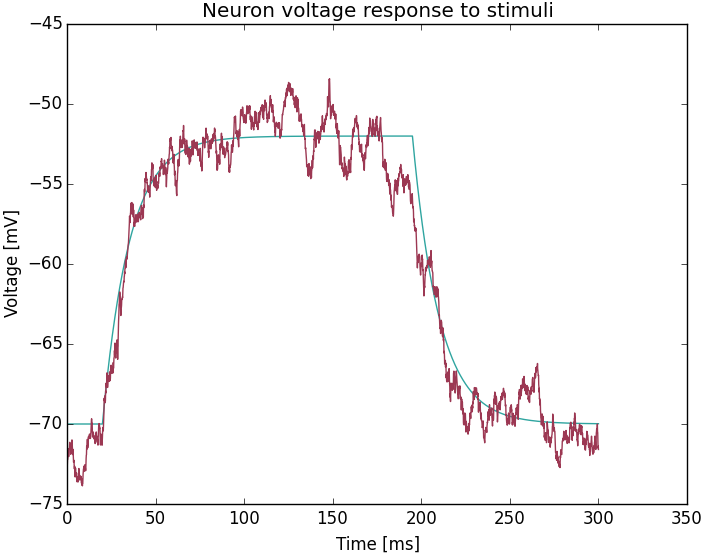
\includegraphics[width=0.37\textwidth]{./fig/Protocol/stims/broad_noised} }}
	\subfloat[rövid áramimpulzusra]{{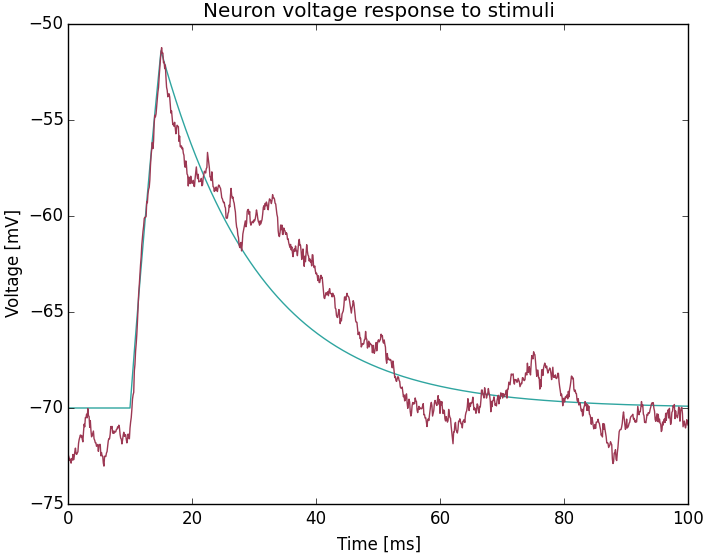
\includegraphics[width=0.37\textwidth]{./fig/Protocol/stims/narrow_noised} }}
	\subfloat[hosszú-rövid áramimpulzusra]{{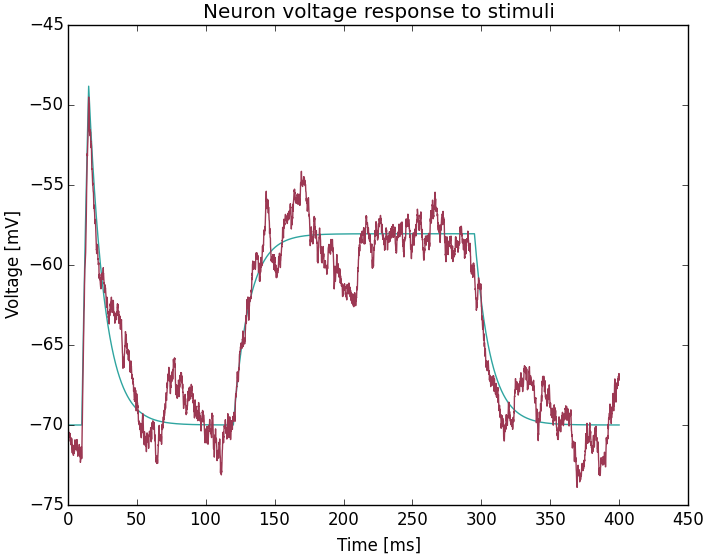
\includegraphics[width=0.37\textwidth]{./fig/Protocol/stims/both_noised} }}
	\\
	\subfloat[$cm$ hosszú impulzusra]{{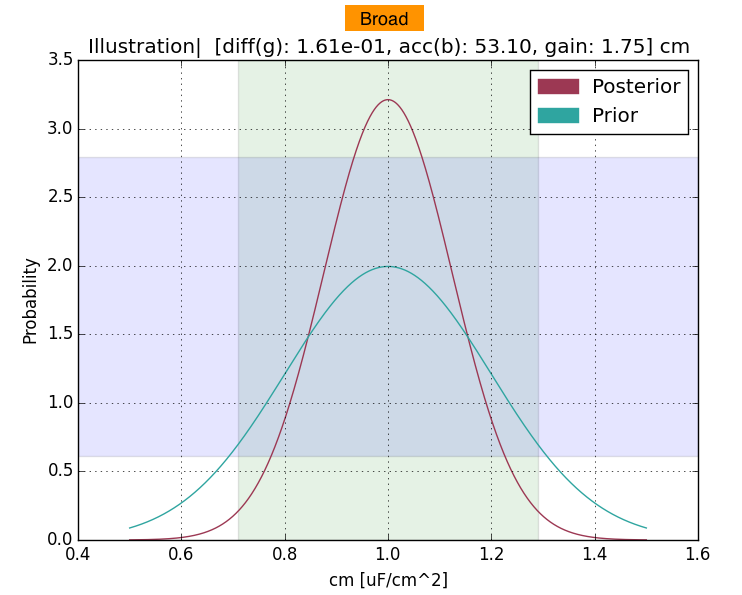
\includegraphics[width=0.37\textwidth]{./fig/Protocol/cm_broad} }}
	\subfloat[$cm$ rövid impulzusra]{{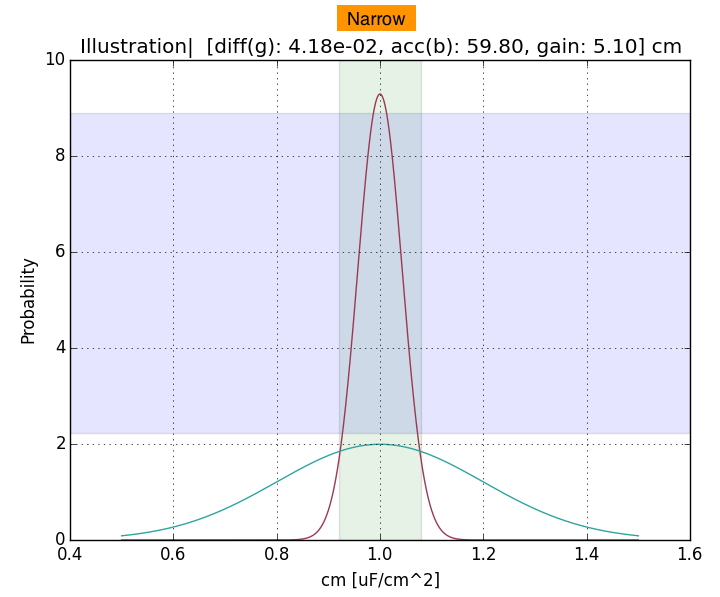
\includegraphics[width=0.37\textwidth]{./fig/Protocol/cm_narrow} }}
	\subfloat[$cm$ hosszú-rövid impulzusra]{{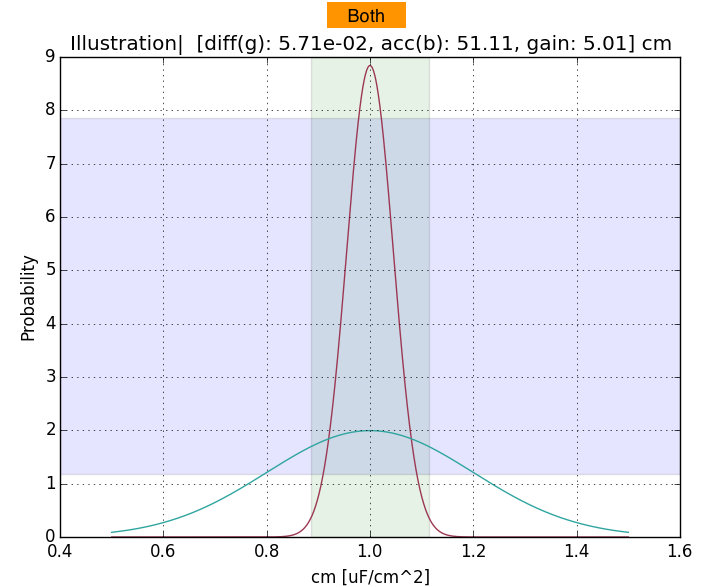
\includegraphics[width=0.37\textwidth]{./fig/Protocol/cm_both} }}
	\\
	\subfloat[$g_{pas}$ hosszú impulzusra]{{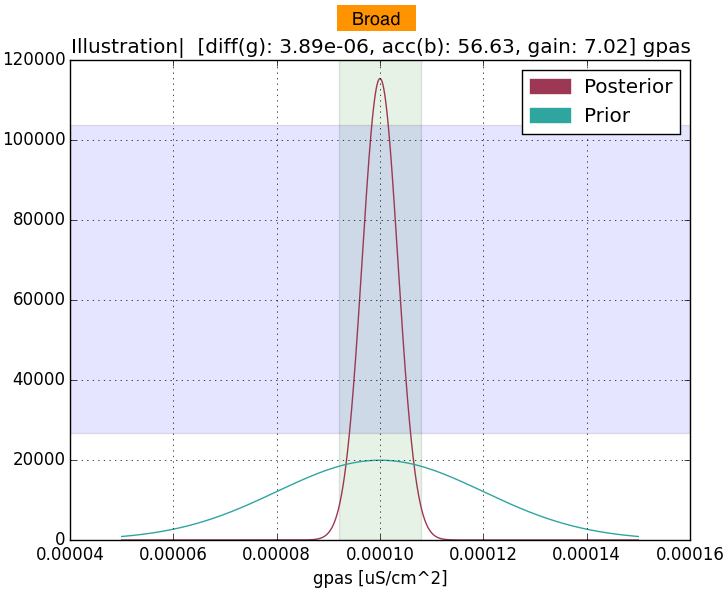
\includegraphics[width=0.37\textwidth]{./fig/Protocol/gpas_broad} }}
	\subfloat[$g_{pas}$ rövid impulzusra]{{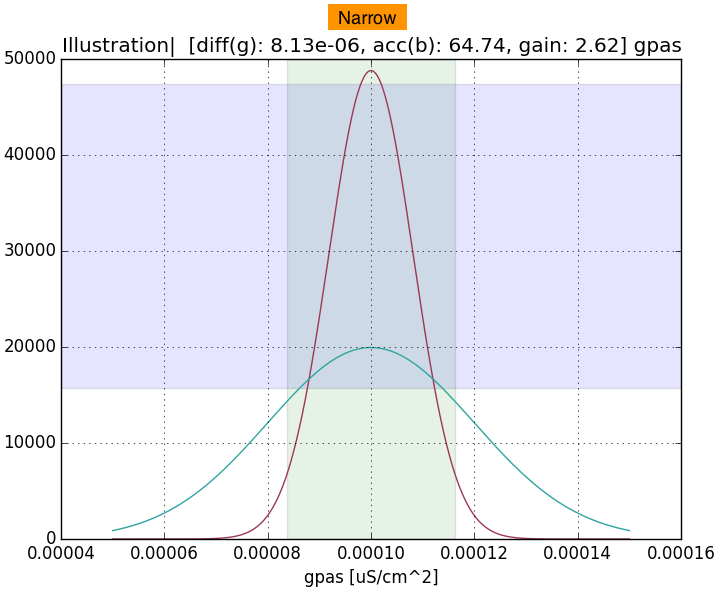
\includegraphics[width=0.37\textwidth]{./fig/Protocol/gpas_narrow} }}
	\subfloat[$g_{pas}$ hosszú-rövid impulzusra]{{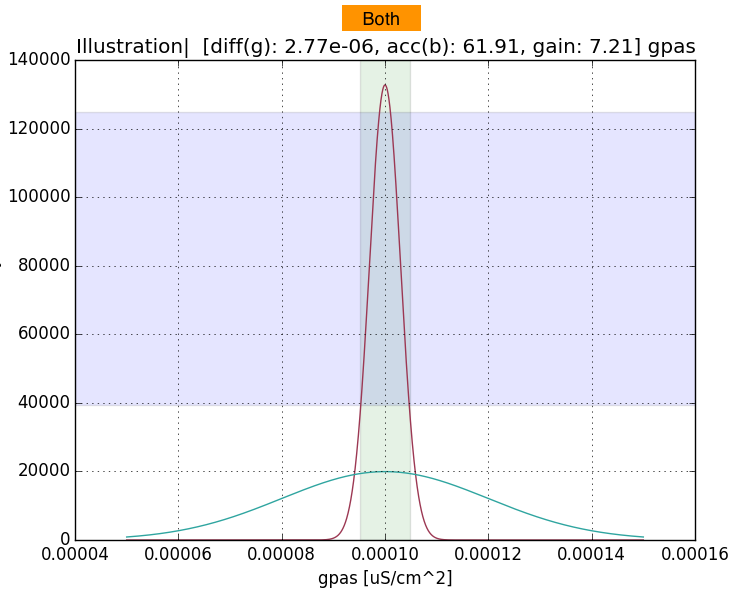
\includegraphics[width=0.37\textwidth]{./fig/Protocol/gpas_both} }}
	\caption[Különböző protokollok és információtartalmuk]{Egykompartmentumos modell különböző áramimpulzusra adott feszültségválaszai láthatóak kékkel, valamint az erre rakott színes zajból előálló szintetikus adatok pirossal az első sorban. Ezek információtartalmát láthatjuk az egyes paraméterekre vonatkozóan a következő sorokban. A második sorban a $cm$ paraméter, a harmadik sorban pedig $g_{pas}$ paraméter eredményei láthatóak.}
	\label{fig:protocol}
\end{figure}



\FloatBarrier
\clearpage
\subsection{Inferencia valódi adatsoron}
Valós (passzív) idegsejt (hosszú és rövid) áramimpulzus bemenetre adott feszültségválaszát mérte az MTA Kísérleti Orvostudományi Kutatóintézetben Nusser Zoltán csapata. Ugyan azokat az elektrofiziológiai méréseket elvégezték sokszor (több mint 500db adatsor született) és a kapott eredményeket átlagolták. Ezután a sejtről egy részletes három dimenziós rekonstrukciót készítettek, mely a korábbi  \ref{fig:morph}-ábrán tekinthető meg. Ezt az idegsejt morfológiát betöltve a \textit{Neuron} programba és elkészítve hozzá a protokollt (sejtbe injektált áramok a megfelelő időpontokban, morfológia és biofizika), megalkottuk a szimulációs modellünk. Itt is a sejttesten történt az ingerlés, valamint azon is mérték a feszültségválaszt. Továbbá csatornablokkolókkal segítségével elérték, hogy a sejt passzív viselkedést mutasson. Így passzív biofizikai beállításokkal használhattuk a számítógépes modellünk. A mérésből származó átlagolt sejtválasz, valamint az idegsejtről készített modellünk szimulációs válasza -- kedvezőtlen paraméterbeállítások mellett -- látható a \ref{fig:exptrace}-ábrán.

\begin{figure}[h!]
	\centering
	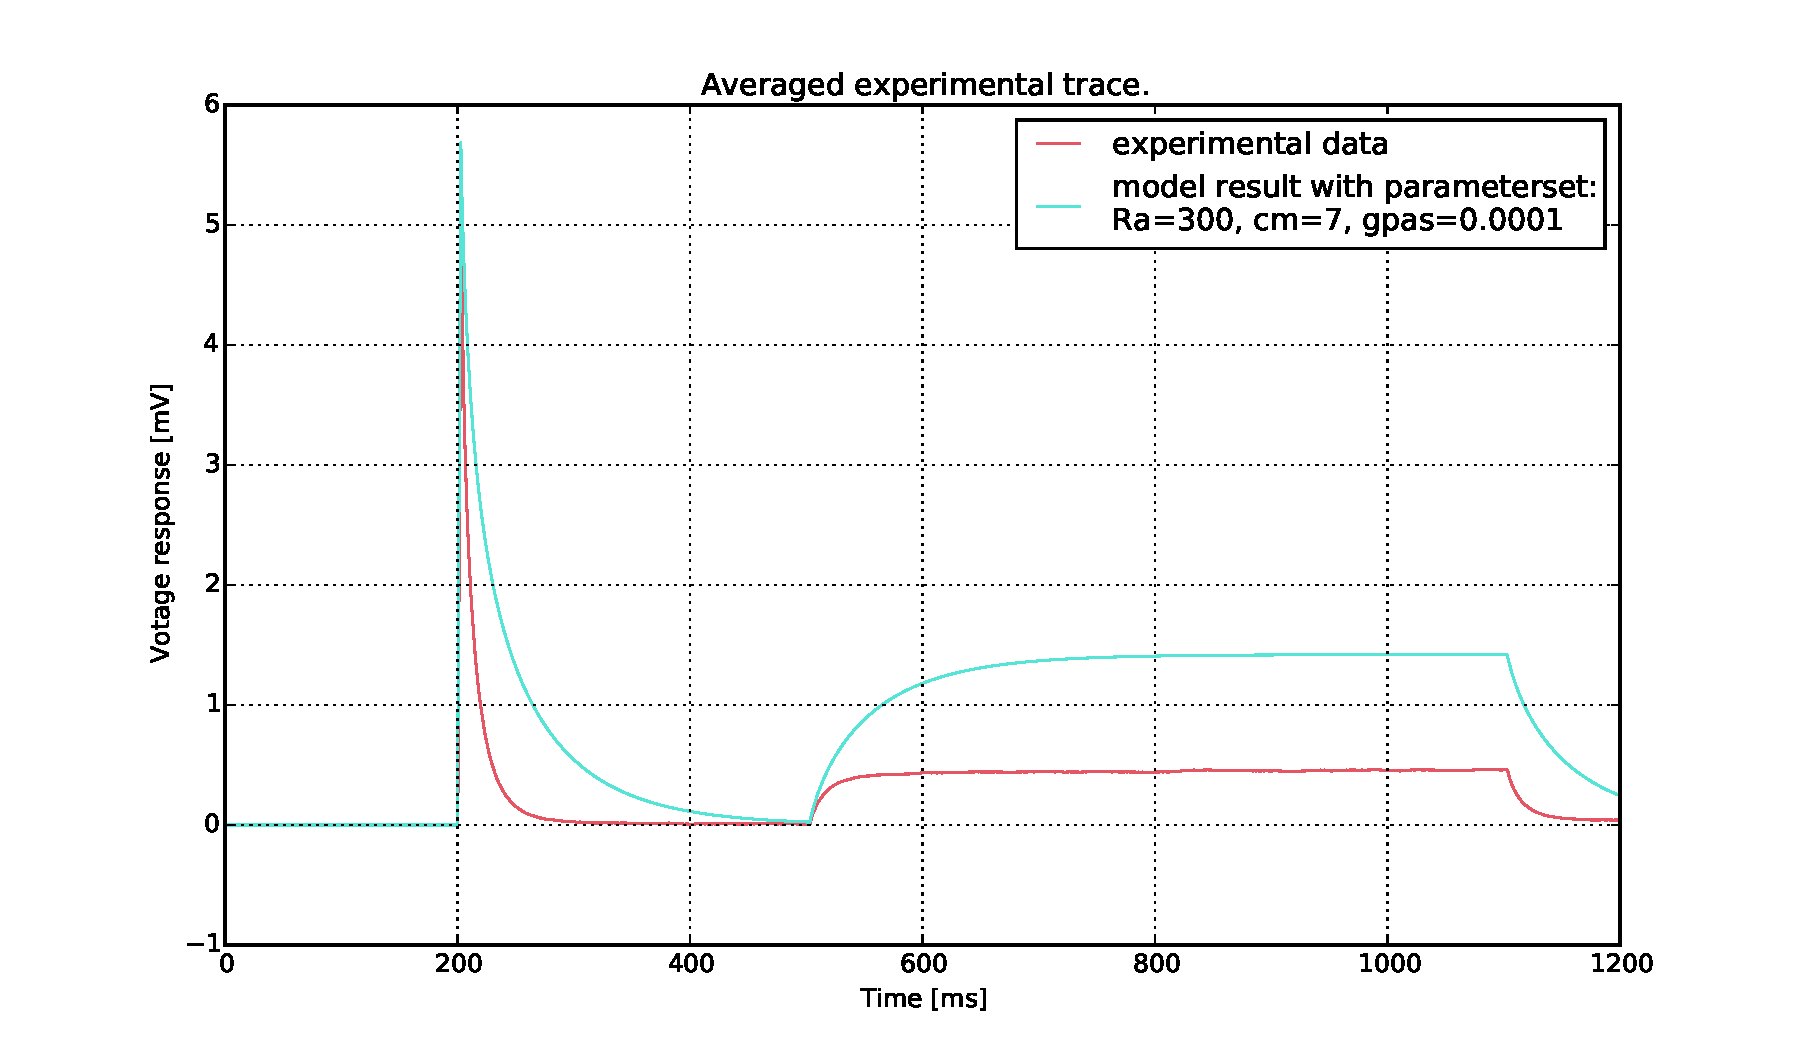
\includegraphics[width=0.9\linewidth]{fig/exp/exptrace.pdf}
	\caption[Valós passzív idegsejt áramimpulzusokra adott feszültségválasza]{Egy valódi passzív idegsejt áramimpulzusokra adott, átlagolt feszültségválasza látható pirossal. A valódi idegsejtről készített szimulációs modell -- rosszul teljesítő paraméterbeállításokkal --  determinisztikus eredménye látható kékkel.}
	\label{fig:exptrace}
\end{figure}

Már csak a kísérleti zaj modellje szükséges az inferencia elvégzéséhez. Ehhez az egyes (baseline) adatsorok autokorrelációs eredményeit átlagoltuk, amely megtekinthető a korábbi \ref{fig:autocorrelation}-ábrán. Erről egyértelműen látszódik, hogy a kísérleti zaj nem modellezhető független fehér zajként, időbeli korreláció figyelhető meg az adatpontok között. Azt vizsgáltuk, hogy az exponenciális lecsengésű autokorrelációval rendelkező színes zajmodellel leírható-e a kísérleti zaj. Ezt úgy tettük, hogy a kiátlagolt autokorrelációs adatokra exponenciális függvényt illesztettünk. Eredményül azt kaptuk, hogy ez a függvény nem illeszkedik jól az adatpontokra. Másrészt az adatsor túl rövid és nem látjuk az aszimptotikus viselkedést\footnote{Feltesszük, hogy az autokorreláció időben nullához tart, azaz egy idő után nem korrelálnak a pontok.} ahhoz, hogy új zajmodellt tudjunk felállítani. Az exponenciális illesztése és egy hipotetikus aszimptotikus viselkedés tekinthető meg \ref{fig:auto_fit}-ábrán.

\begin{figure}[h!]
	\centering
	\subfloat[$exp$ fit]{{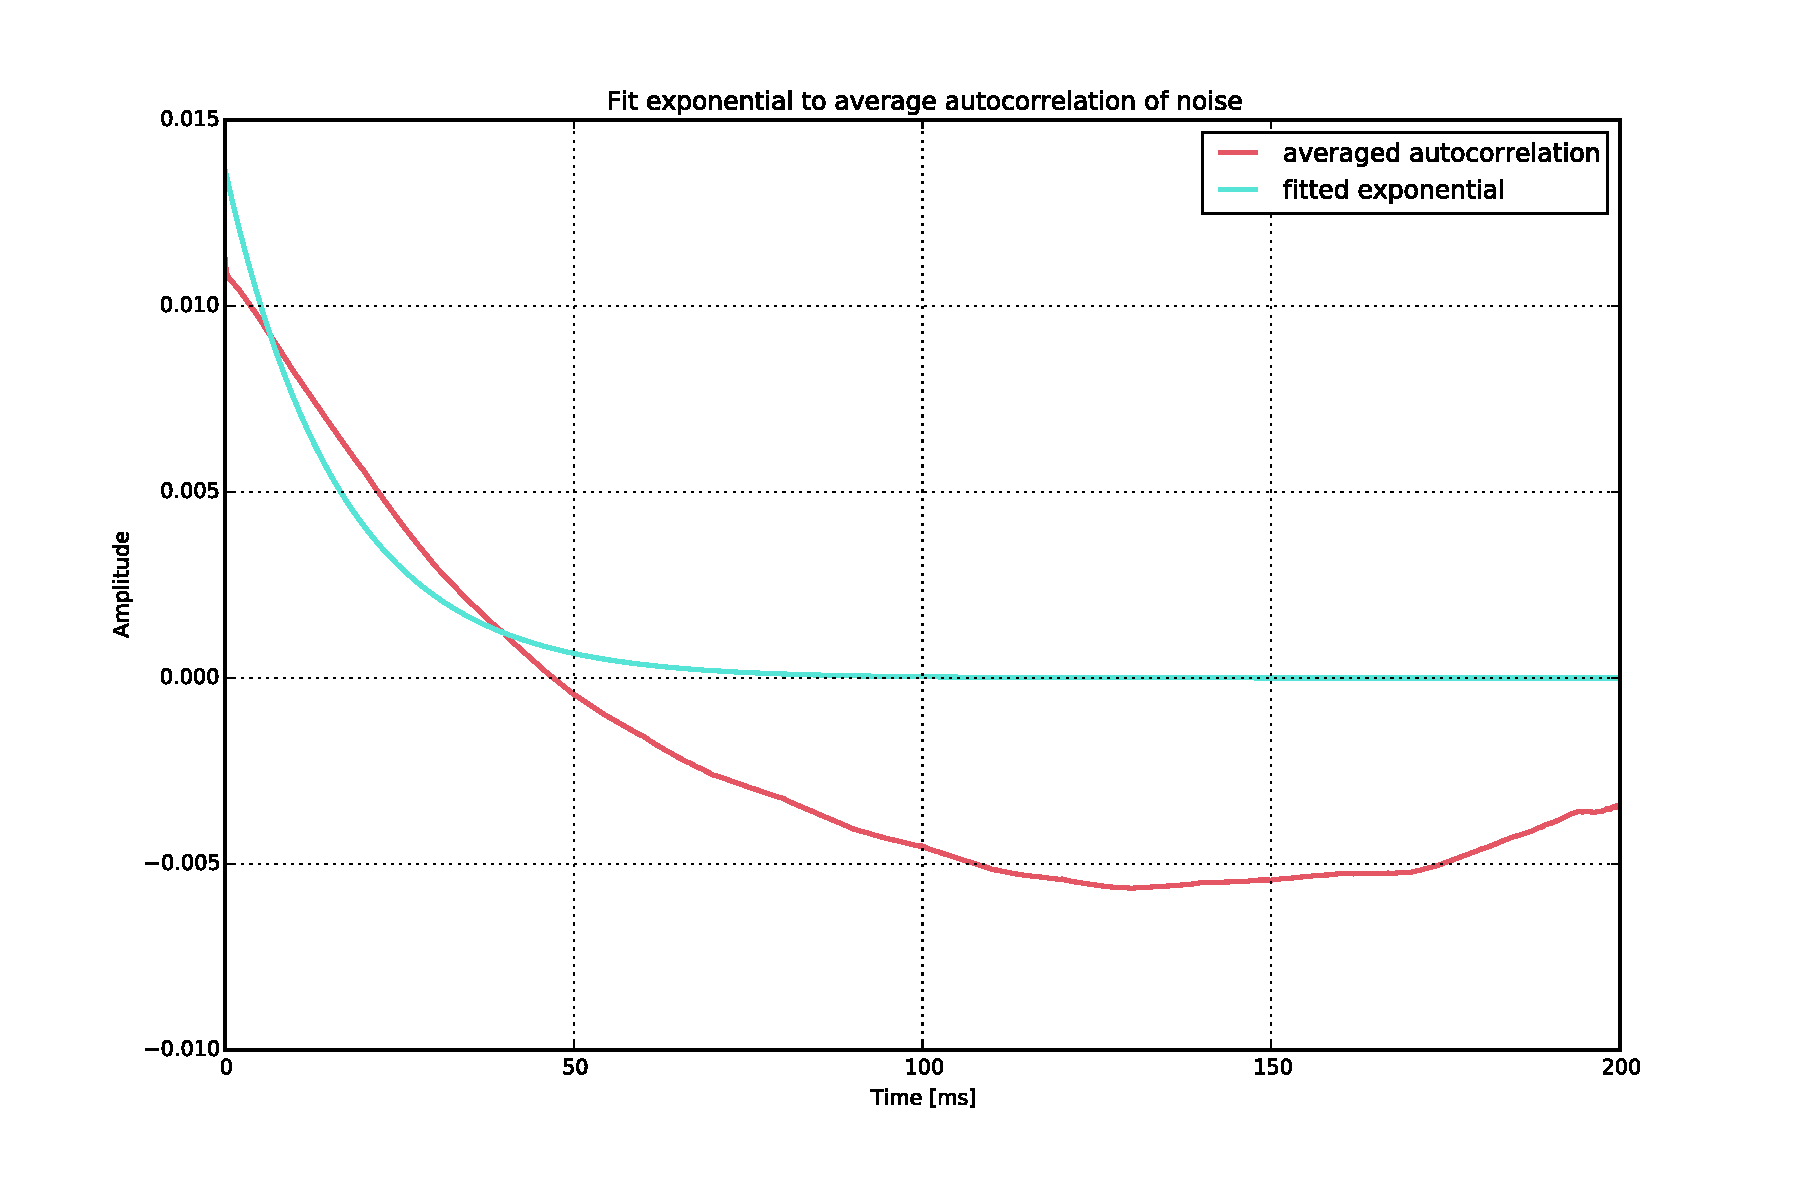
\includegraphics[width=0.5\textwidth]{./fig/exp/exponential_fit.pdf} }}
	\subfloat[$exp-gauss$ fit]{{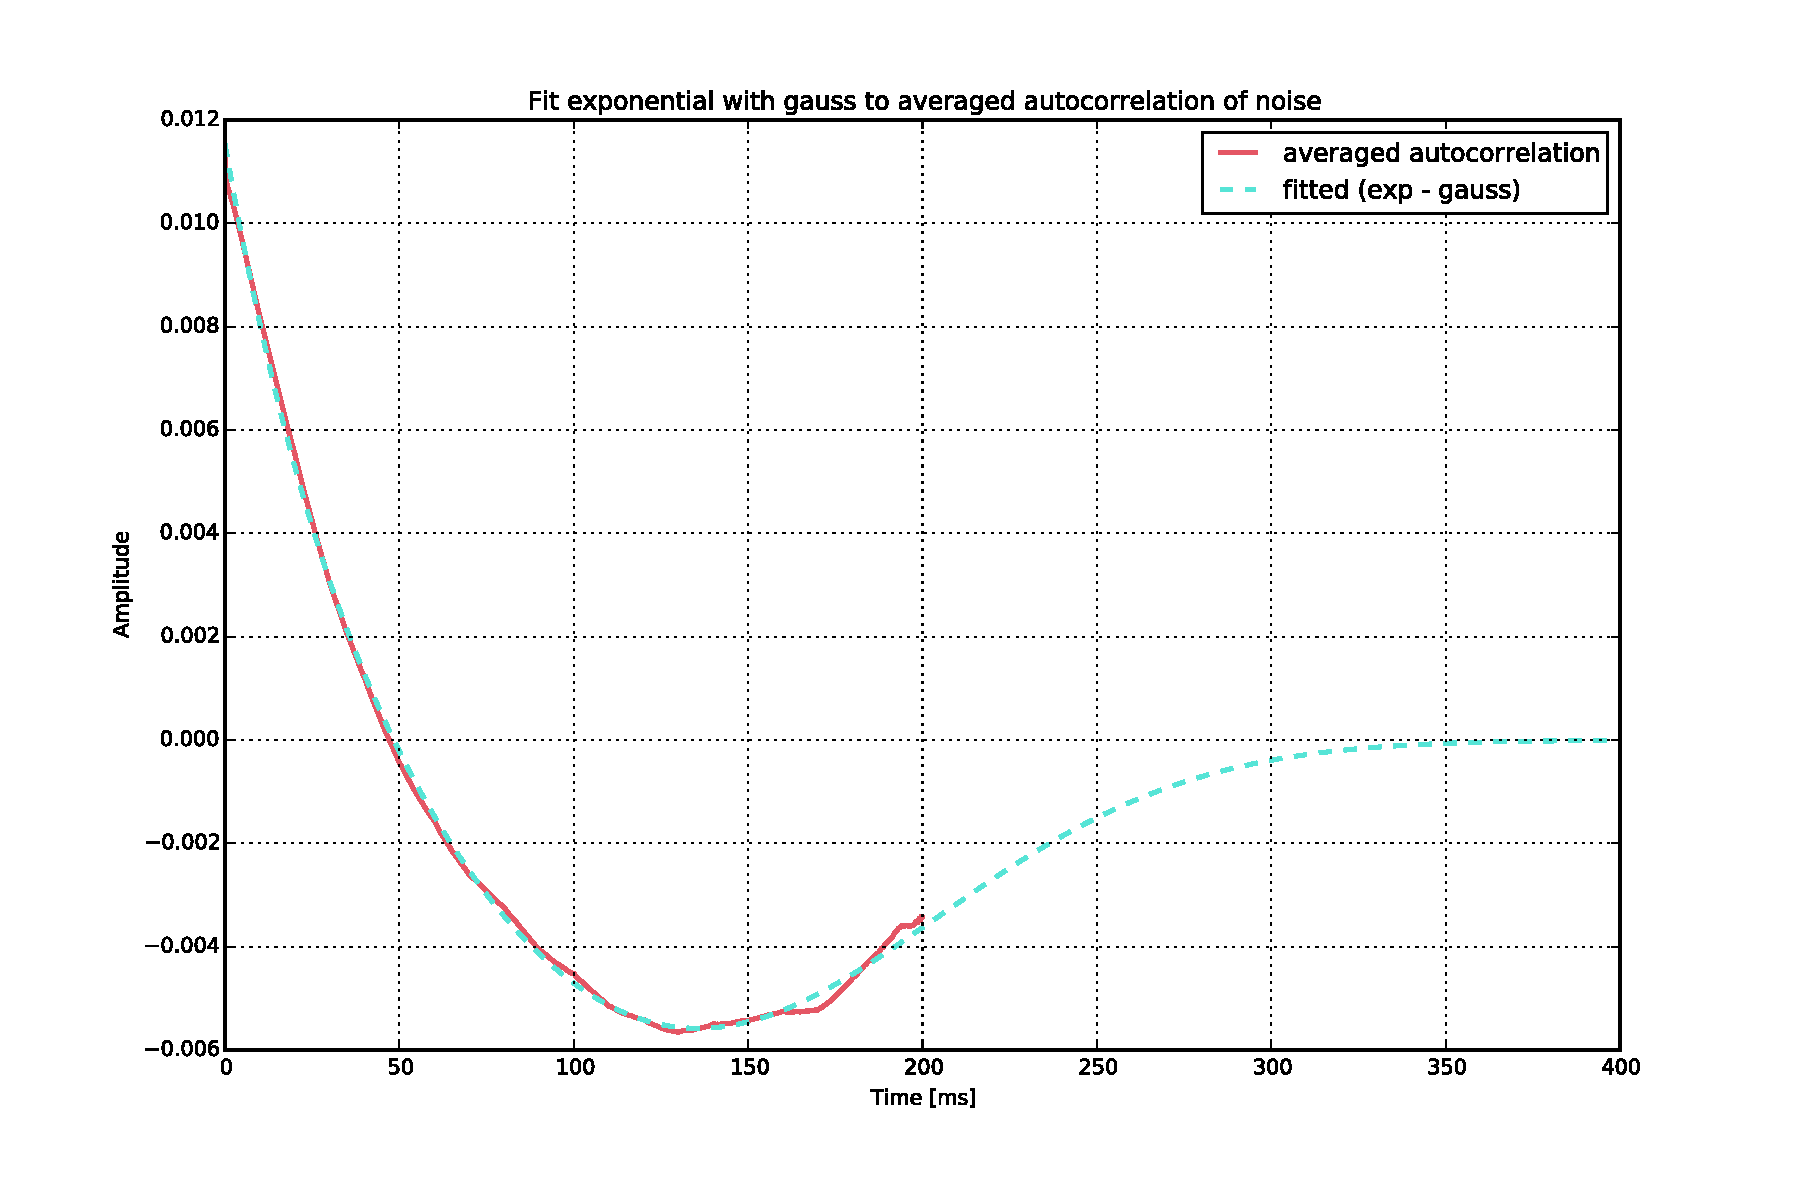
\includegraphics[width=0.5\textwidth]{./fig/exp/exp_and_gauss.pdf} }}
	\caption[Illesztés az autokorrelációs adatokra]{\textbf{(a)}: Kiátlagolt autokorrelációs adatokra exponenciális illesztése. Az illeszkedés rossz, az adatok a negatívba is lemennek. \textbf{(b):} Másrészt az adatsor túl rövid, az aszimptotikus viselkedés nem látható. Itt is egy exponenciálist illesztettünk kiegészítve egy Gauss-görbével: minimum $400-500 [ms]$-os basile kellene az aszimptotikus viselkedéshez. Az is elképzelhető feltevés, hogy a függvény oszcillálva tart nullába...}
	\label{fig:auto_fit}
\end{figure}

Ebből fakadóan fehér zajt feltételezve alkalmaztuk a paraméterbecslést az átlagolt adatsorra. Az átlagolás következtében viszont erősen lecsökkent a zaj szórása\footnote{Nem csak a fehér zaj, de bármilyen korreláló zaj is kiátlagolódik, mivel maguk az adatsorok függetlenek.}, így mi egy kis -- az eddigi vizsgálatainknál használttal összemérhető -- amplitúdójú fehér zajt alkalmaztunk. Ezekből kifolyólag az eredményünk azt fogja jellemezni, hogy ez a komplex térbeli kiterjedésű idegsejtmodell mennyire érzékeny a paraméterekre. Az inferenciát egyszerre mind a három passzív paraméteren ($R_a$, $cm$, $g_{pas}$) végeztük. Az \textit{Optimizer}\cite{friedrich2014flexible} paraméteroptimalizációs szoftverrel előre megkerestük a legjobban illeszkedő paraméterkombinációt, majd az ezt körülölelő paramétertér egy felosztását kiértékeltük, elvégeztük az inferenciát. Az egyes eredmények a \ref{fig:result}-ábrán láthatók, valamint ezek összefoglalása a~\ref{fig:fullplot_res}-ábrán. Az ábrákról szépen látszódik, hogy a paraméterek együttesen határozzák meg a modell jó illeszkedését. Ez különösen a $g_{pas}$ paraméterrel való együttes eloszlásoknál látszódik, ugyanis ha rögzítem az egyik paramétert egy nagyobb valószínűségű helyen, ahhoz tartozik a másik paraméter egy olyan beállítása, mellyel a modell jól teljesít és ezek a nagy valószínűségű helyek egy éles vonalon helyezkednek el.

Összességében megállapíthatjuk, hogy valós elektrofiziológiai adatokra és idegsejtmodellekre is szépen működik a módszerünk. Viszont a megjelenő kísérleti zaj még kérdéses, hosszabb adatsorra van szükség és további elemezést kíván.

\begin{figure}[h!]
	\centering
	\subfloat[$R_a-cm$ likelihood]{{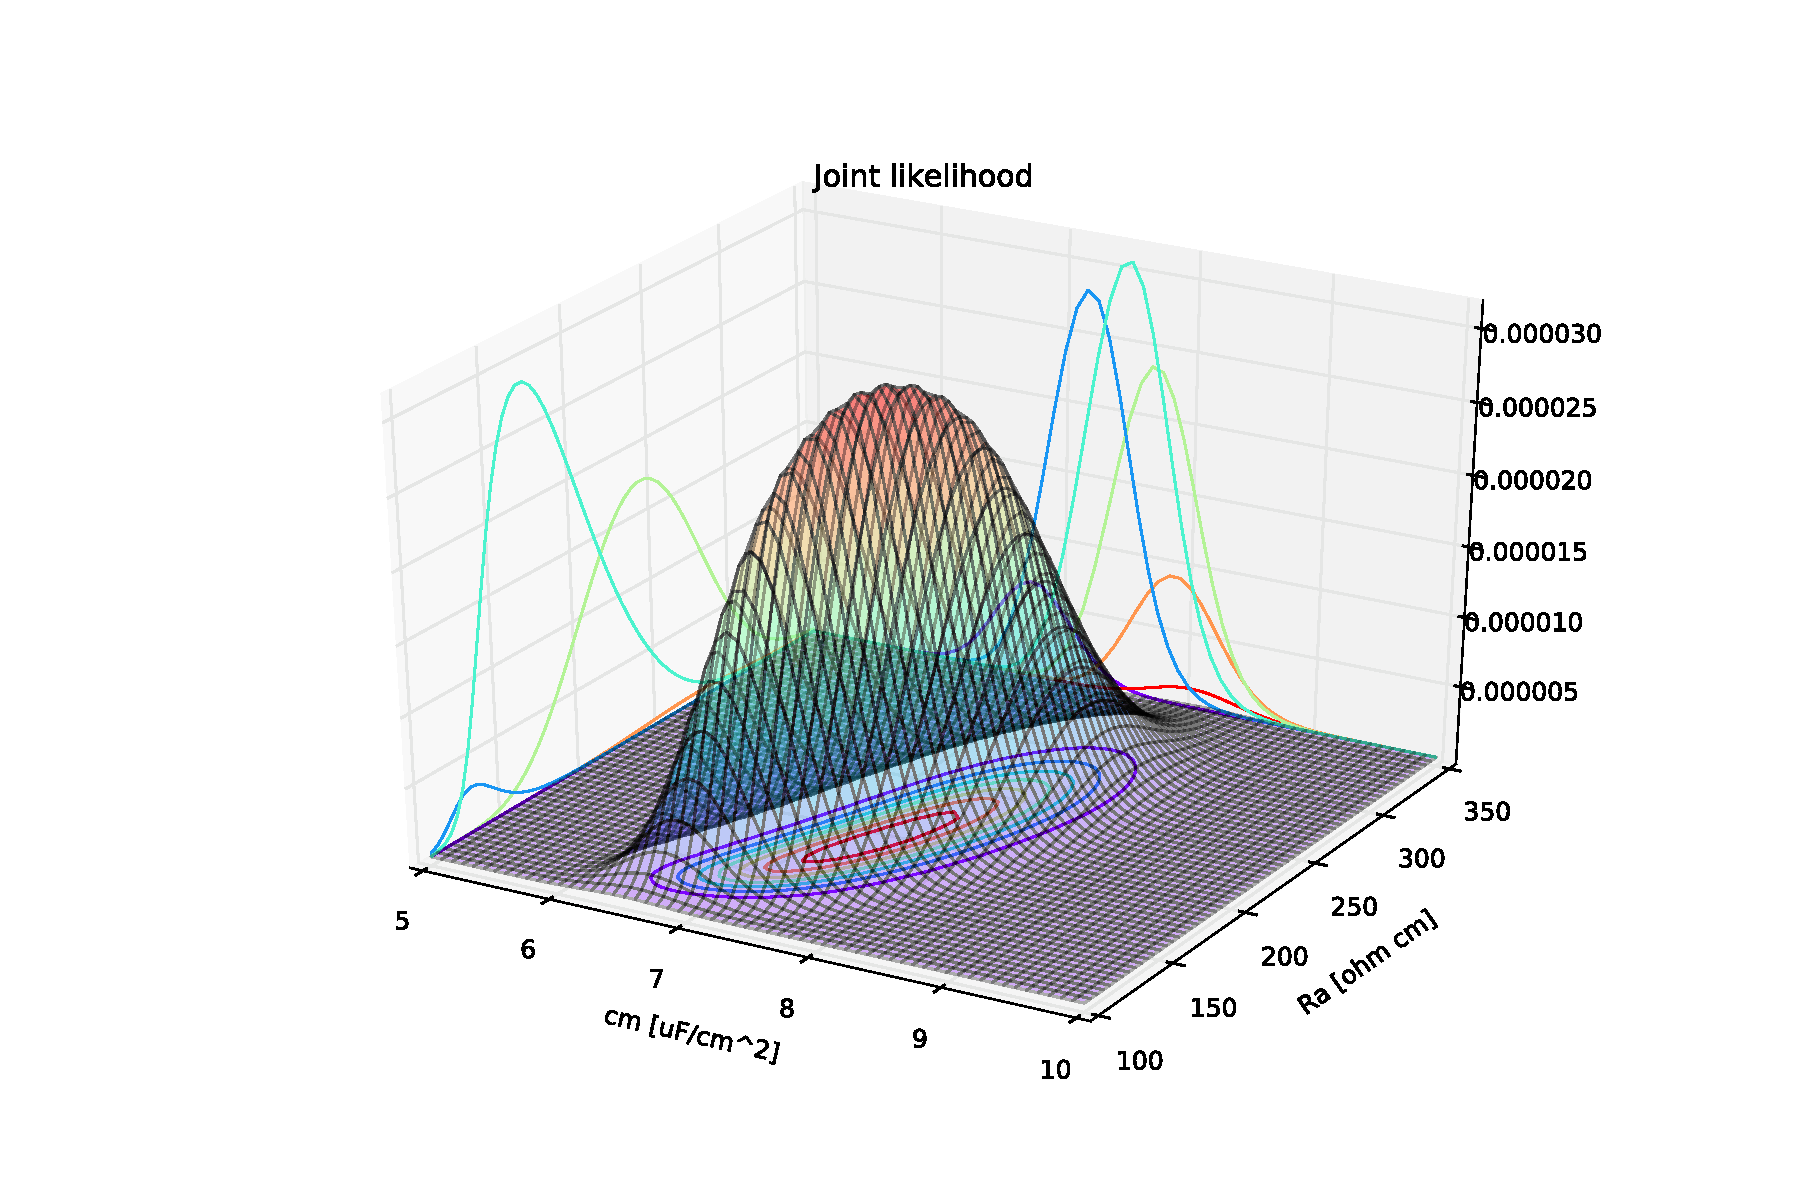
\includegraphics[width=0.37\textwidth]{./fig/exp/L_Ra-cm(0).pdf} }}
	\subfloat[$R_a-g_{pas}$ likelihood]{{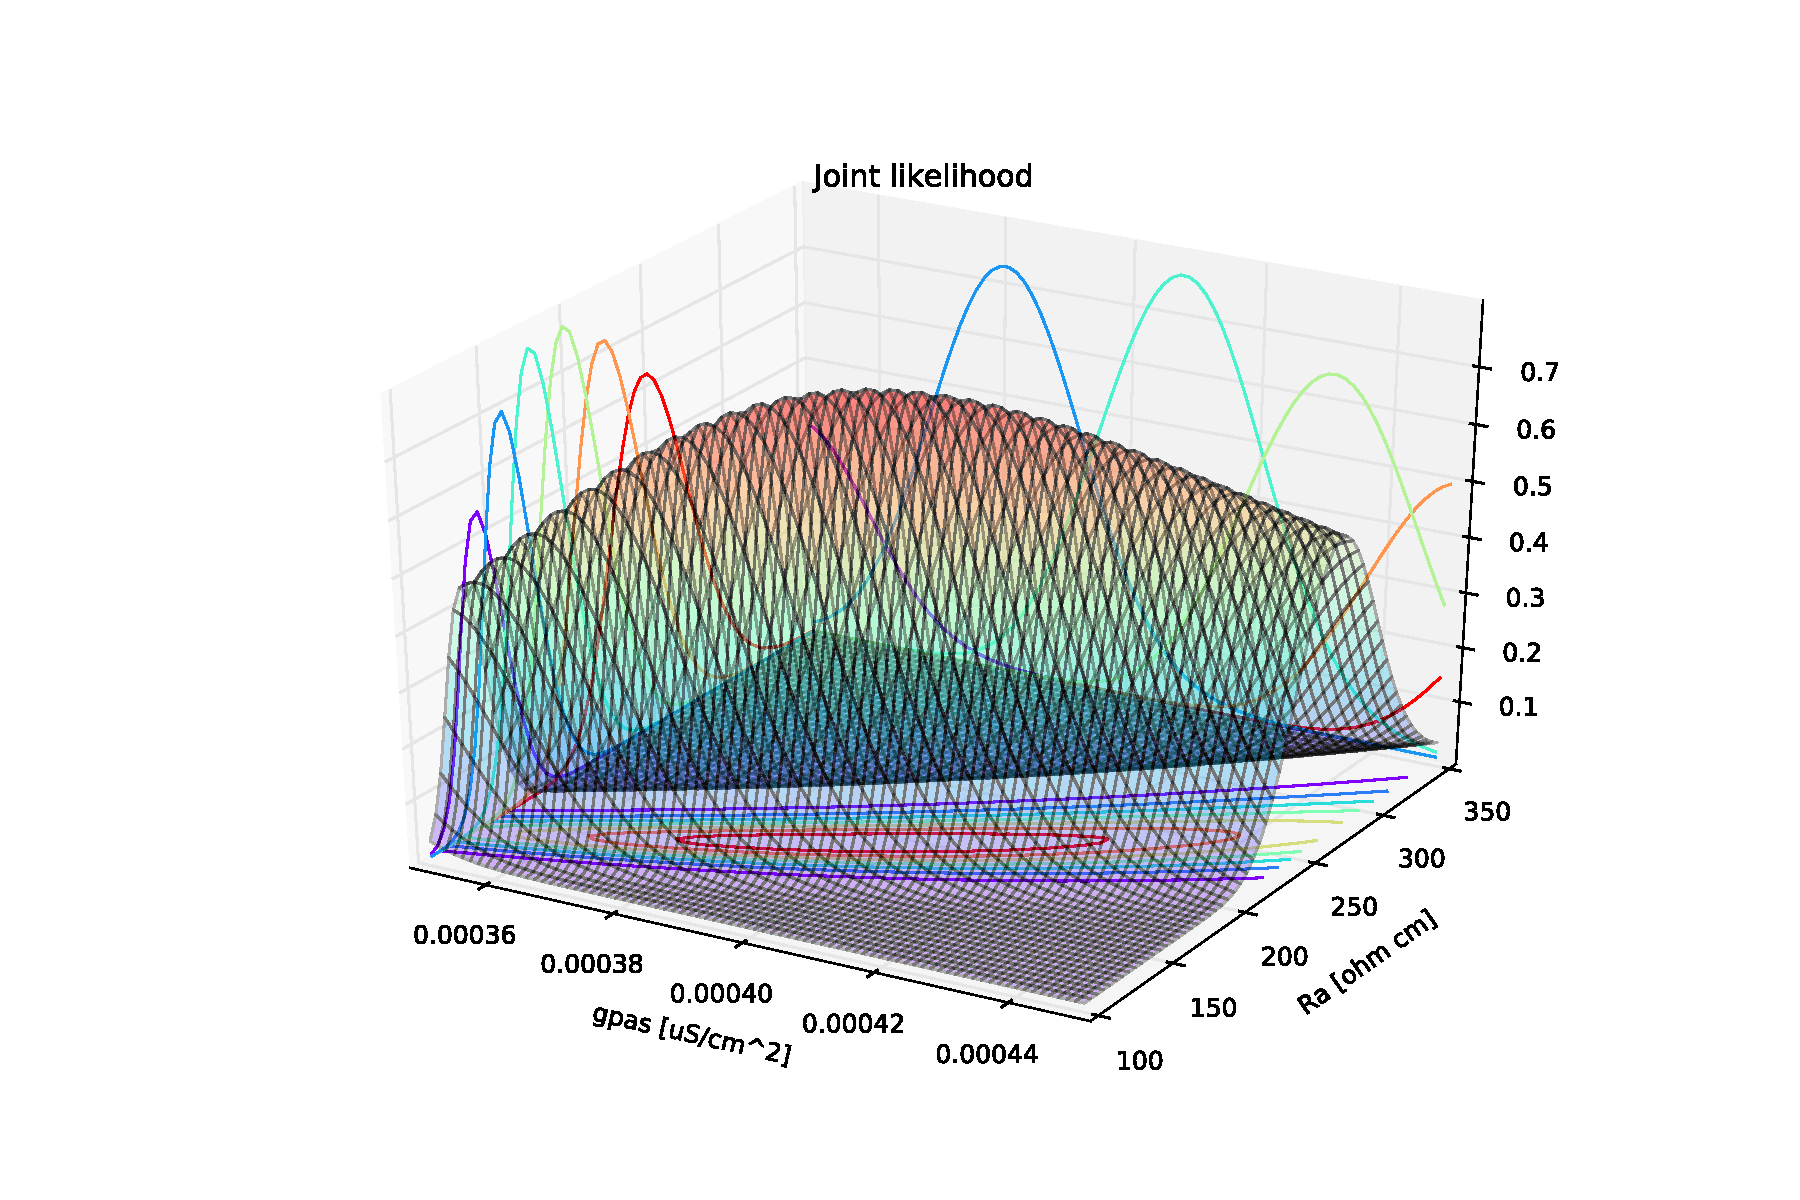
\includegraphics[width=0.37\textwidth]{./fig/exp/L_Ra-gpas(0).pdf} }}
	\subfloat[$cm-g_{pas}$ likelihood]{{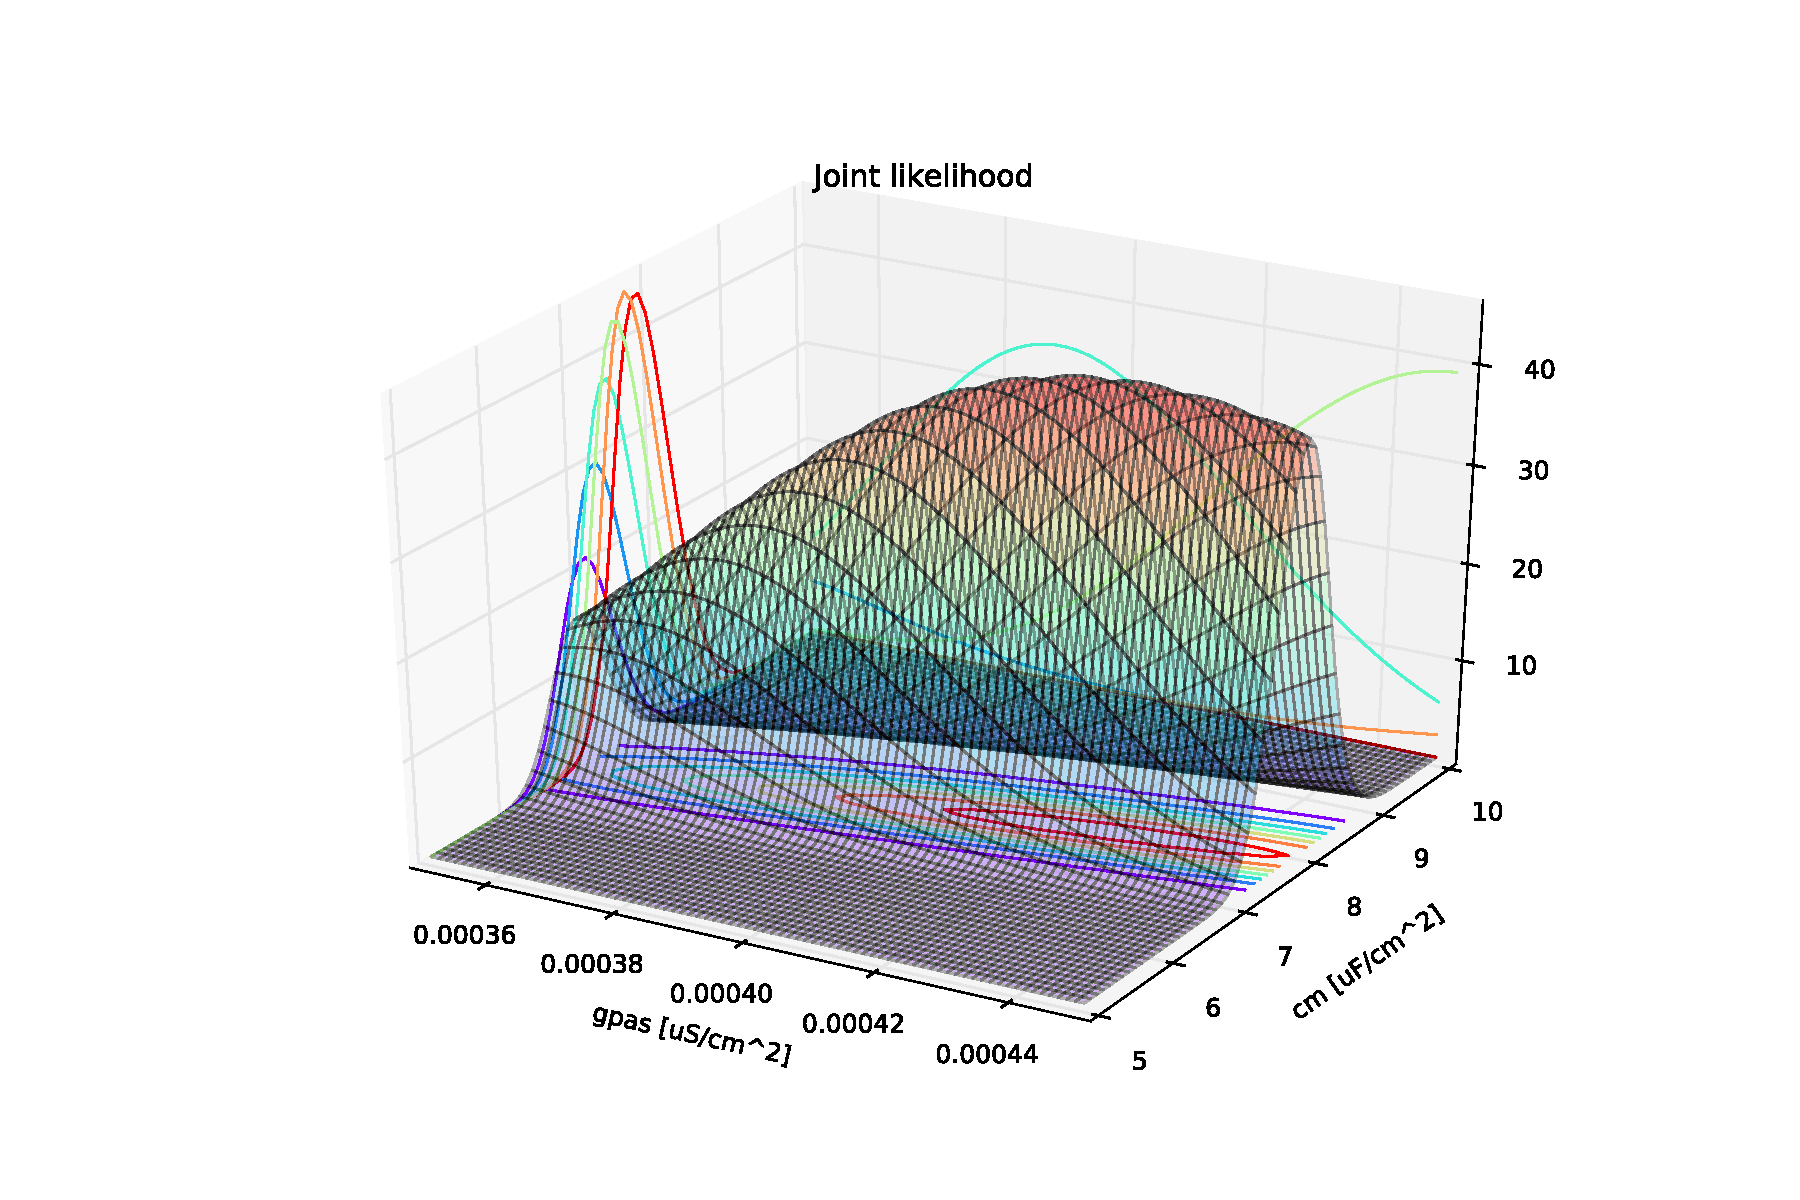
\includegraphics[width=0.37\textwidth]{./fig/exp/L_cm-gpas(0).pdf} }}
	\\
	\subfloat[$R_a$ likelihood]{{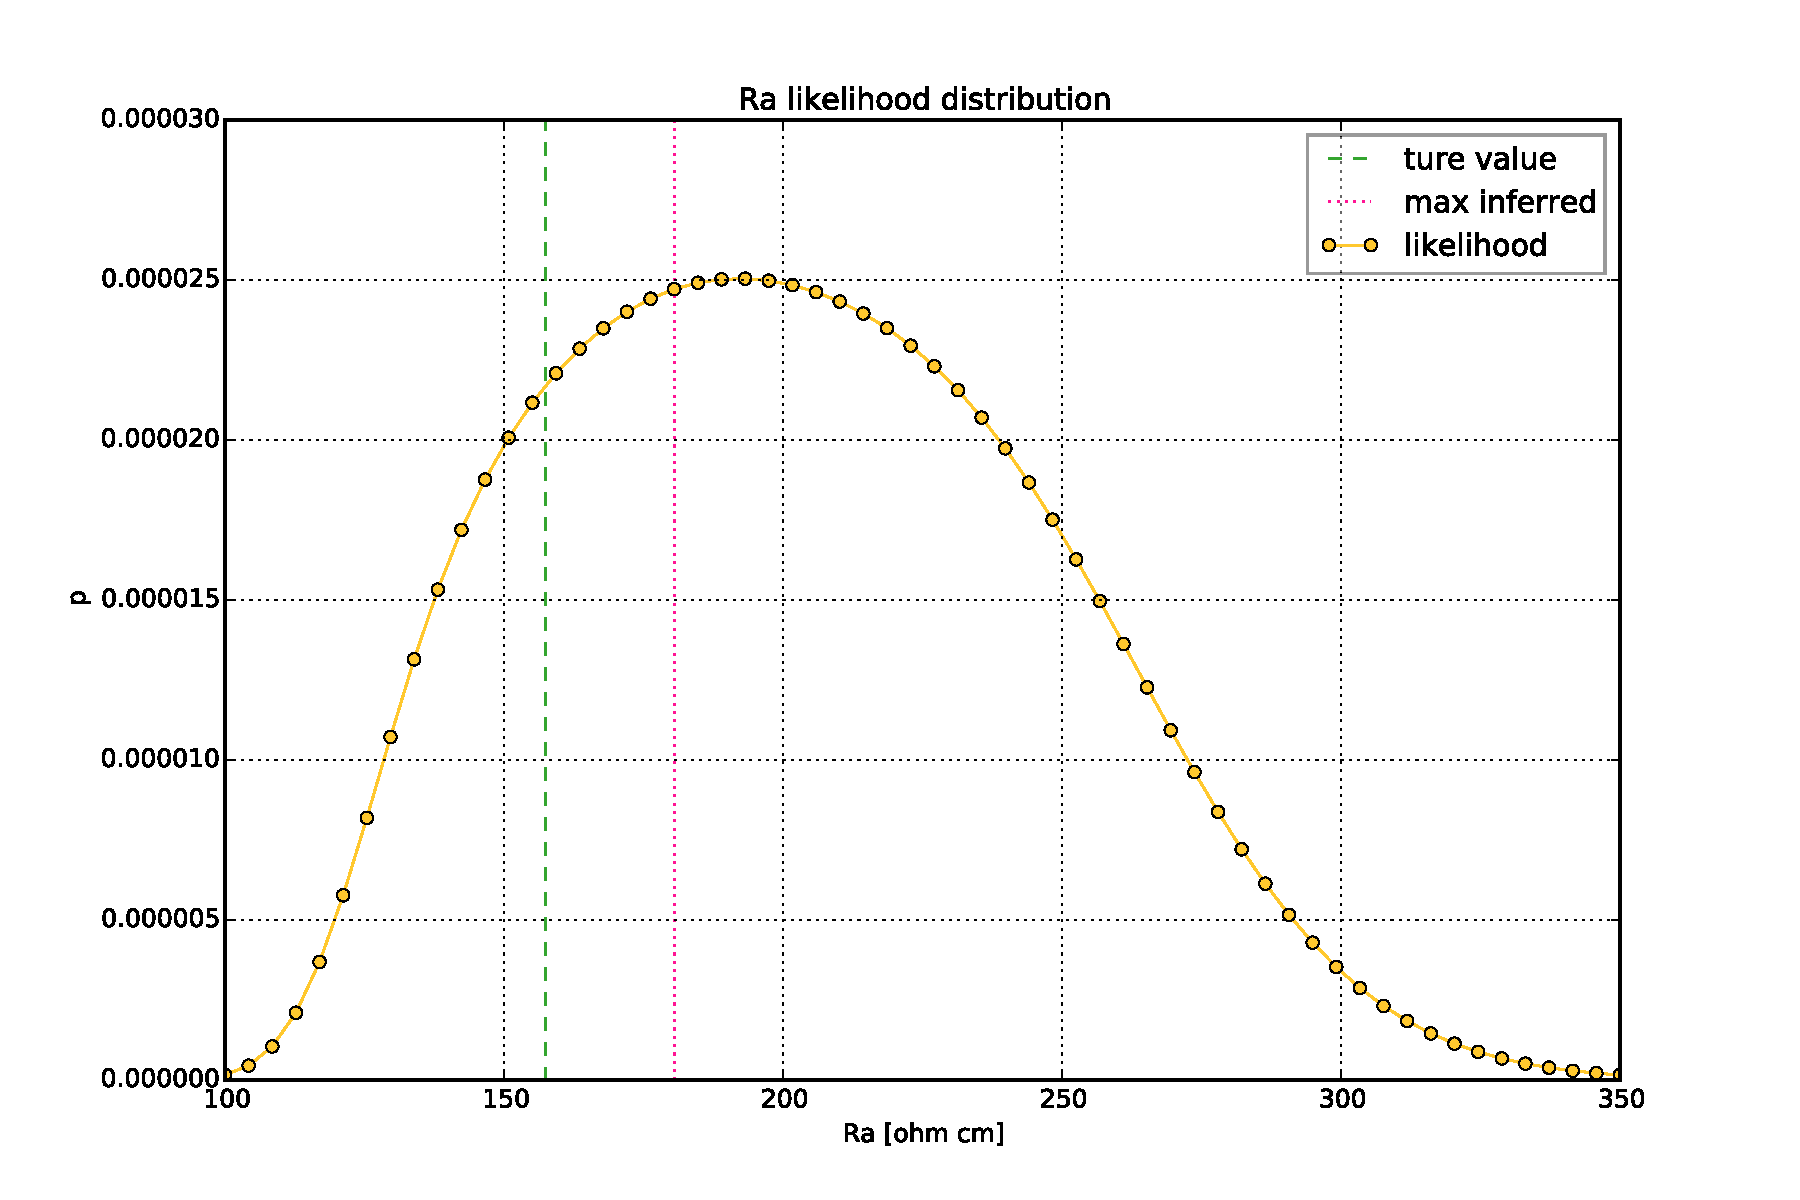
\includegraphics[width=0.37\textwidth]{./fig/exp/Ra_L(0).pdf} }}
	\subfloat[$cm$ likelihood]{{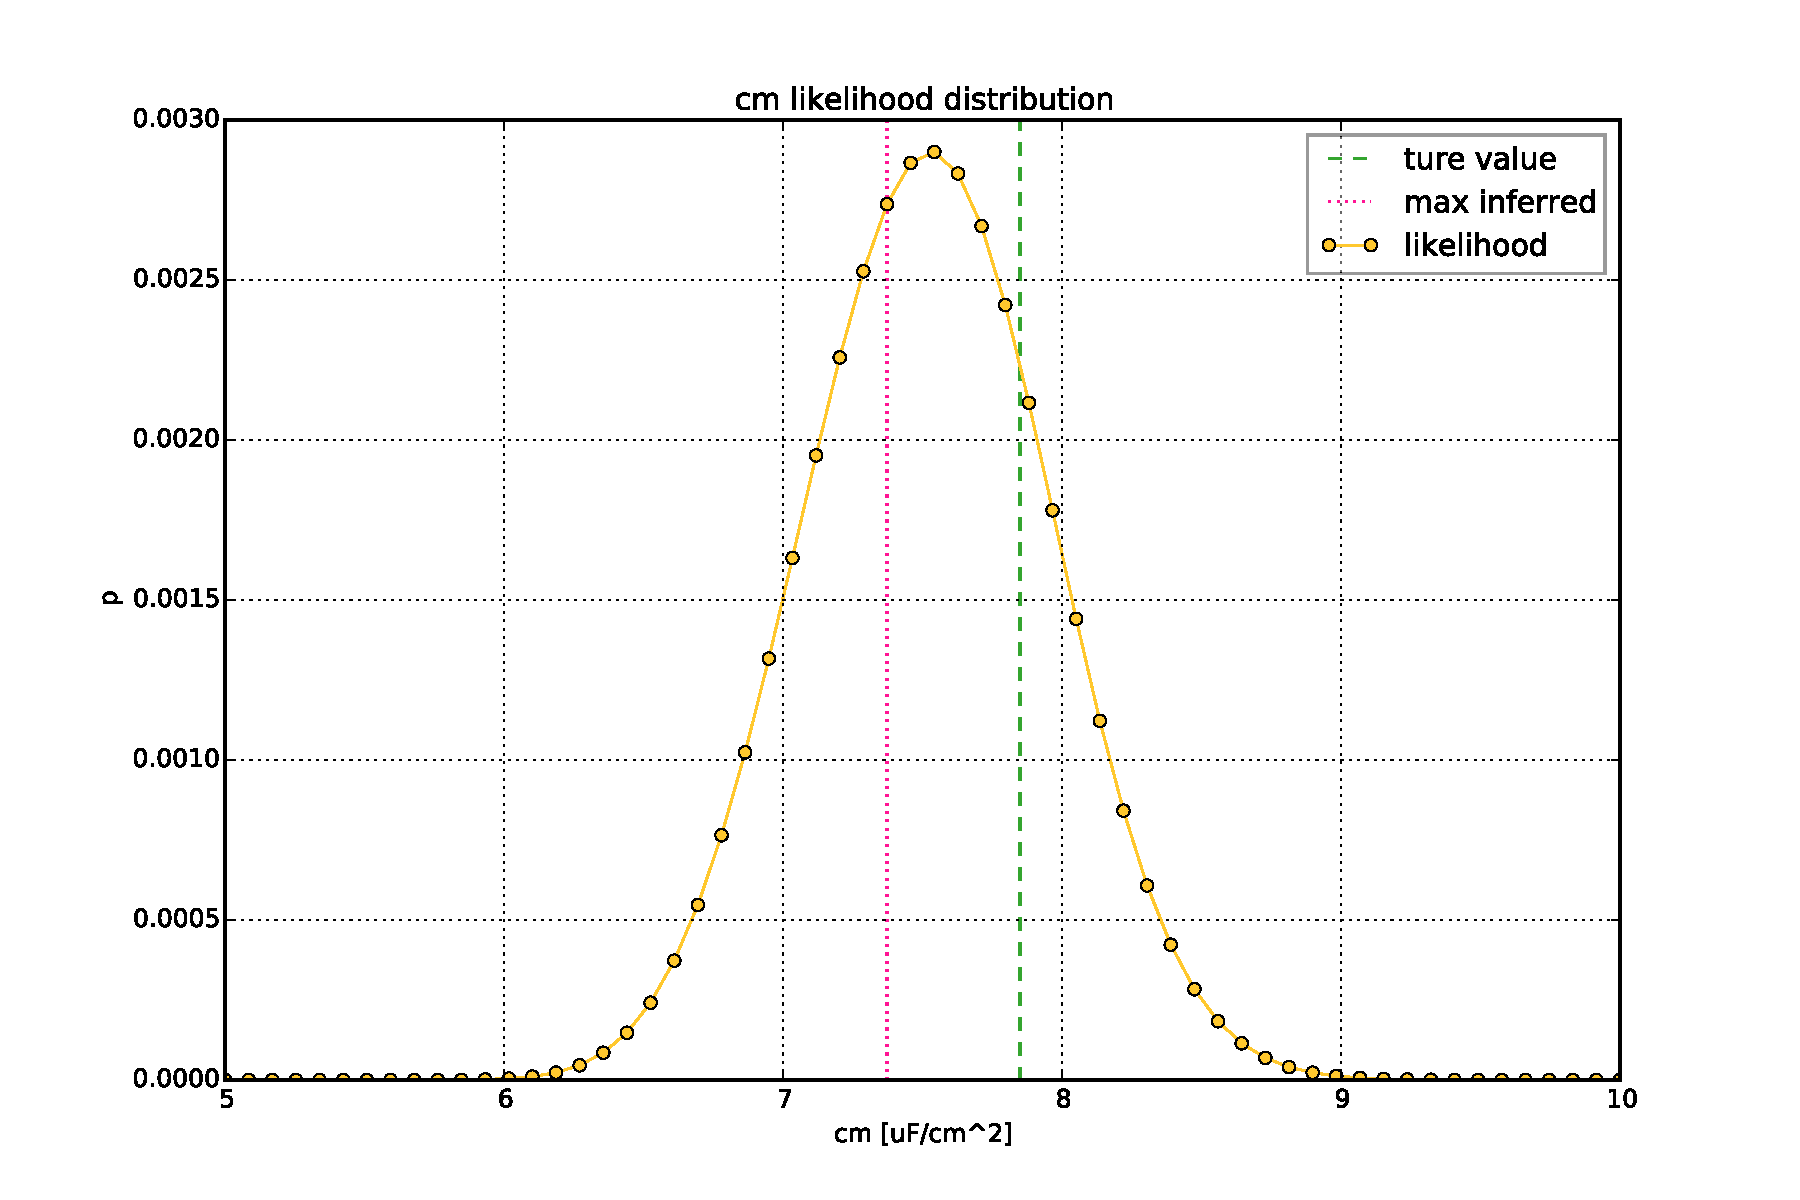
\includegraphics[width=0.37\textwidth]{./fig/exp/cm_L(0).pdf} }}
	\subfloat[$g_{pas}$ likelihood]{{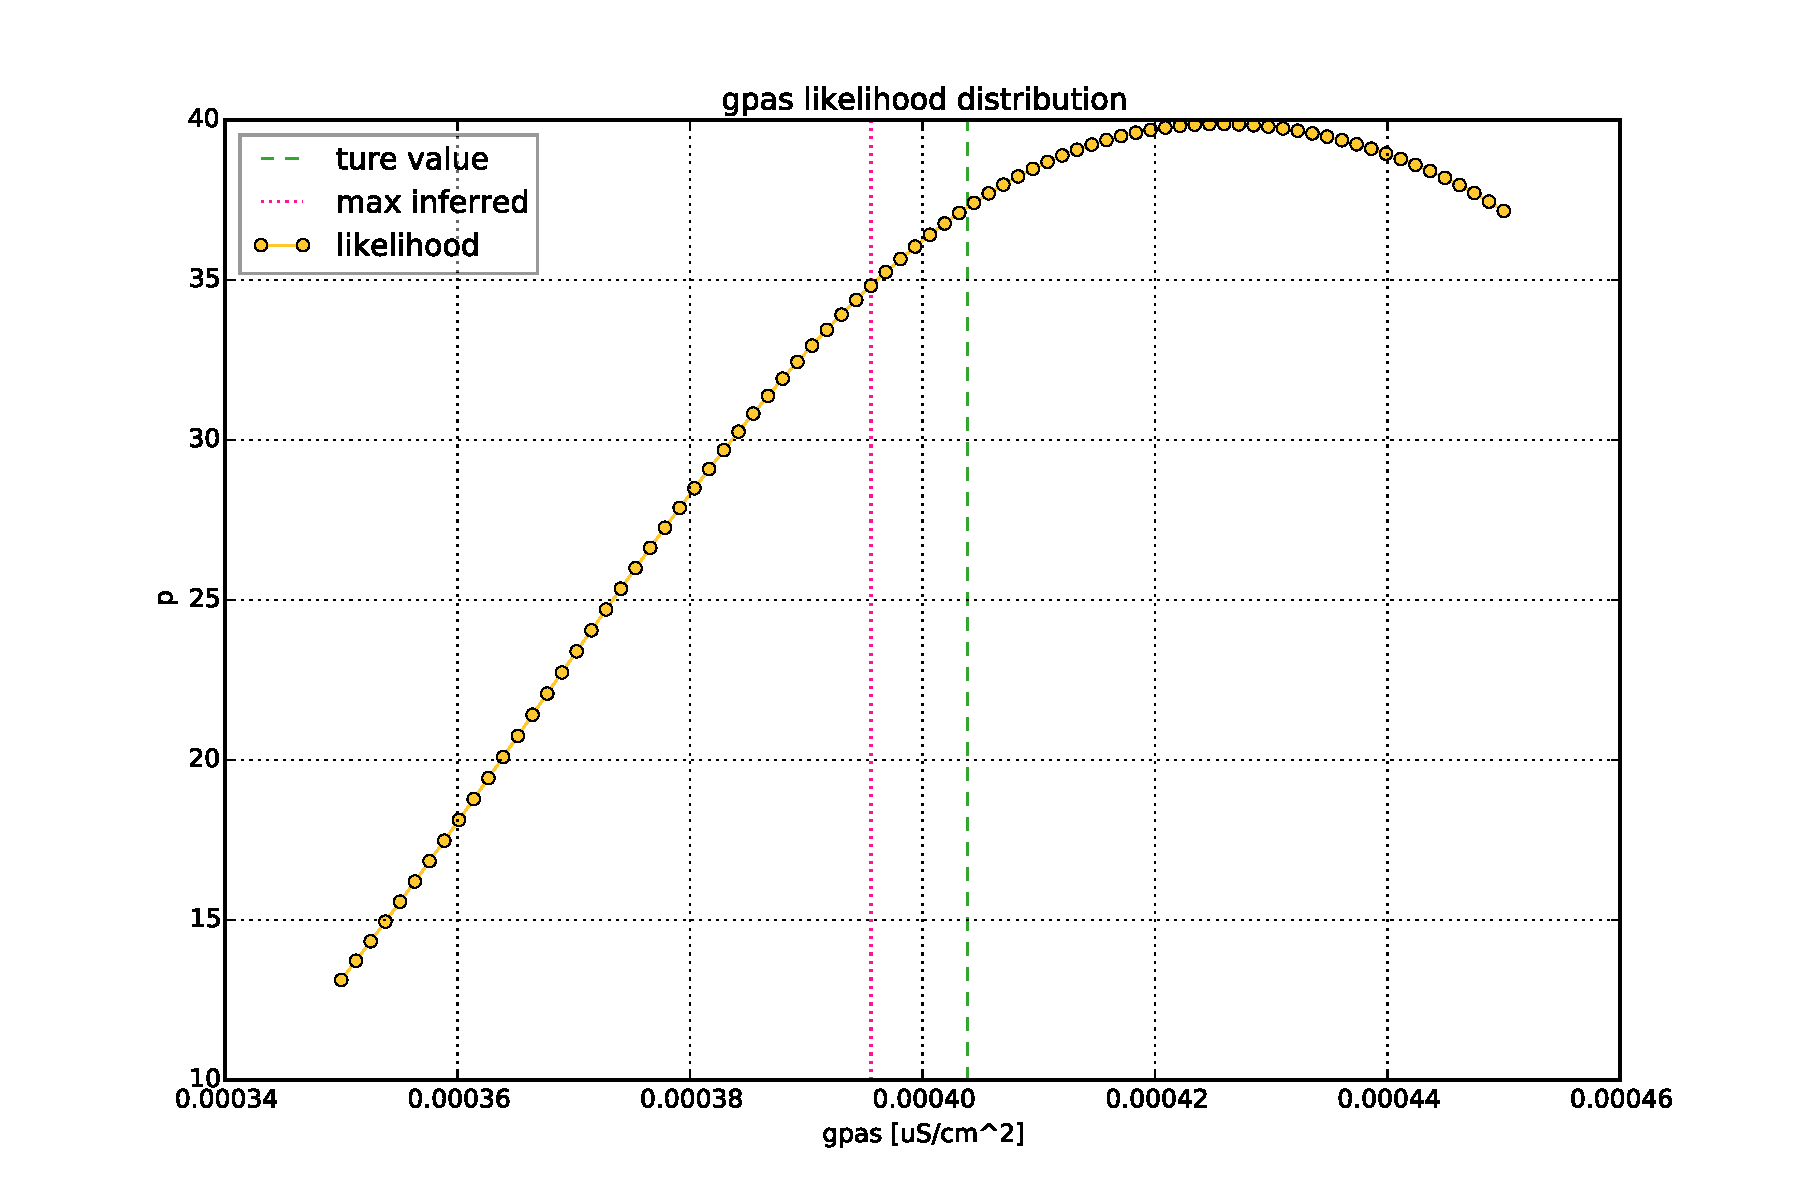
\includegraphics[width=0.37\textwidth]{./fig/exp/gpas_L(0).pdf} }}
	\\
	\subfloat[$R_a-cm$ poszterior]{{\includegraphics[width=0.37\textwidth]{./fig/exp/P_Ra-cm(0).pdf} }}
	\subfloat[$R_a-g_{pas}$ poszterior]{{\includegraphics[width=0.37\textwidth]{./fig/exp/P_Ra-gpas(0).pdf} }}
	\subfloat[$cm-g_{pas}$ poszterior]{{\includegraphics[width=0.37\textwidth]{./fig/exp/P_cm-gpas(0).pdf} }}
	\\
	\subfloat[$R_a$ poszterior]{{\includegraphics[width=0.37\textwidth]{./fig/exp/Ra_P(0).pdf} }}
	\subfloat[$cm$ poszterior]{{\includegraphics[width=0.37\textwidth]{./fig/exp/cm_P(0).pdf} }}
	\subfloat[$g_{pas}$ poszterior]{{\includegraphics[width=0.37\textwidth]{./fig/exp/gpas_P(0).pdf} }}
	\caption[Valós kísérleti adatsoron végzett inferencia eredményei]{A valós kísérleti adatsoron végzett inferencia eredményei láthatók.}
	\label{fig:result}
\end{figure}

\begin{figure}[h!]
	\centering
	\subfloat[Likelihood eredmények]{{\includegraphics[width=\textwidth]{./fig/exp/fullplot_L(0).pdf} }}\\
	\subfloat[Poszterior eloszlás]{{\includegraphics[width=\textwidth]{./fig/exp/fullplot_P(0).pdf} }}
	\caption[Valós kísérleti adatsoron végzett inferencia összefoglaló ábrája]{Az összefoglaló ábra látható a paraméterbecslés eredményéről, valós passzív idegsejtre.}
	\label{fig:fullplot_res}
\end{figure}



\pagebreak
% Konklúziós
\section{Következtetés}

\pagebreak
\appendix
\section{Függelék}
\subsection{Mintavételezés}

\subsection{Időlépések}

\pagebreak
\section*{Köszönetnyilvánítás} 
Először is szeretném megköszönni a témavezetőmnek, Káli Szabolcsnak a rengeteg segítségét, útmutatását és türelmes hozzáállását, ami nélkül ez a dolgozat nem jöhetett volna létre. Nagyon kellemes tapasztalat volt a vele történő munka és a vele töltött idő.


Szeretném megköszönni továbbá édesanyám és keresztapám anyagi támogatását, fáradozását annak érdekében, hogy megteremtsék a megfelelő hátteret a tanulmányaim elvégzéséhez.

Valamint köszönöm barátaimnak az ösztönzésüket, különösön Demeter Márton Csabának, volt kollégiumi szobatársamnak, akitől sokat tanulhattam. Végezetül köszönöm barátnőmnek, Kósa Rékának, hogy végig mellettem állt.

% Bibliográfia
\pagebreak
\bibliographystyle{plain}
\bibliography{references.bib}
\end{document}

